\documentclass[11pt]{article}

% if you need to pass options to natbib, use, e.g.:
%\PassOptionsToPackage{numbers}{natbib}
\usepackage[colorlinks,linkcolor=blue,filecolor=blue,citecolor=magenta,urlcolor=blue]{hyperref}
\usepackage{bm,amsmath,amsthm,amssymb,multicol,algorithmic,algorithm,enumitem,graphicx,subfigure}
\usepackage{xargs}
\usepackage{xcolor}
\usepackage{wrapfig}
\usepackage{stmaryrd}
\usepackage{natbib}
% \usepackage[english]{babel}

% ready for submission
\usepackage{neurips_2021}
\def\M{\mathcal{M}}
\def\A{\mathcal{A}}
\def\Z{\mathcal{Z}}
\def\S{\mathcal{S}}
\def\D{\mathcal{D}}
\def\R{\mathcal{R}}
\def\P{\mathcal{P}}
\def\K{\mathcal{K}}
\def\E{\mathbb{E}}
\def\F{\mathfrak{F}}
\def\l{\boldsymbol{\ell}}

\newtheorem{Fact}{Fact}
\newtheorem{Lemma}{Lemma}
\newtheorem{Prop}{Proposition}
\newtheorem{Theorem}{Theorem} 
\newtheorem{Def}{Definition}
\newtheorem{Corollary}{Corollary}
\newtheorem{Conjecture}{Conjecture}
\newtheorem{Property}{Property}
\newtheorem{Observation}{Observation}
\newtheorem{Exa}{Example}
\newtheorem{assumption}{H\!\!}
\newtheorem{Remark}{Remark}
\newtheorem*{Lemma*}{Lemma}
\newtheorem*{Theorem*}{Theorem}
\newtheorem*{Corollary*}{Corollary}
 
\newcommand{\eqsp}{\;}
\newcommand{\beq}{\begin{equation}}
\newcommand{\eeq}{\end{equation}}
\newcommand{\eqdef}{\mathrel{\mathop:}=}
\def\EE{\mathbb{E}}
\newcommand{\norm}[1]{\left\Vert #1 \right\Vert}
\newcommand{\pscal}[2]{\left\langle#1\,|\,#2 \right\rangle}
\def\major{\mathsf{M}}
\def\rset{\ensuremath{\mathbb{R}}}

\begin{document}
\title{On Distributed Adaptive Optimization with Gradient Compression}

\author{
Xiaoyun Li \\
  Cognitive And Computing Lab\\
  Baidu Research\\
  Beijing, USA \\
  \texttt{xiaoyun@baidu.com} 
   \And
  Belhal Karimi \\
  Cognitive And Computing Lab\\
  Baidu Research\\
  Beijing, China \\
  \texttt{v_karimibelhal@baidu.com} 
   \And
  Ping Li \\
  Cognitive And Computing Lab\\
  Baidu Research\\
  Beijing, China \\
  \texttt{liping@baidu.com} \\
}

\date{\today}

\maketitle

\vspace{-0.1in}
\begin{abstract}
We study \algo, a distributed optimization framework based on gradient averaging and adaptive AMSGrad algorithm. Gradient compression is applied to reduce the communication in the gradient transmission process, whose bias is corrected by the tool of error feedback. Our convergence analysis of \algo\ shows two novel results in adaptive optimization: (i) like SGD, error feedback can also fix the convergence issue of compressed gradients for adaptive method, achieving same convergence rate as the full-gradient counterpart; (ii) distributed \algo\ has a linear speedup w.r.t. the number of local workers. Numerical experiments are conducted to justify the theoretical findings, and demonstrate significant communication reduction of the proposed method. Since \algo\ is simple and efficient in both communication and memory, it can serve as a convenient distributed training protocol for adaptive methods.

\end{abstract}

\vspace{-0.05in}
\section{Introduction}\label{sec:introduction}
\vspace{-0.05in}

Deep neural network has achieved the state-of-the-art learning performance on numerous AI applications, e.g., computer vision~\cite{Proc:GAN_NIPS14,Proc:Resnet_CVPR16,CV_review18}, Natural Language Processing~\cite{Proc:Graves_ICASSP13,NLP_review18,sentiment_review18}, Reinforcement Learning~\cite{Arxiv:MnihKSGAWR13,AlphaGo_17} and recommendation systems~\cite{Proc:Covington_2016,Article:Wei_2017}. 
With the sheet size of data observations and the increasing complexity of deep neural networks, standard single-machine training procedures encounter at least two major challenges:
\begin{itemize}
    \item Due to the limited computing power of a single-machine, processing the massive number of data samples takes a long time --- training is too slow. Many real-world applications can not even afford spending that much time on training.
  
    \item In many practical scenarios, data are typically stored in multiple servers, possibly at different locations, due to the storage constraints (massive user behavior data, Internet images, etc.) or privacy reasons~\cite{Proc:Chang18}. 
    Hence, transmitting data among servers might be costly.
\end{itemize}
\textit{Distributed learning} framework~\cite{Proc:Dean_NIPS12} has been a common training strategy to tackle the above two issues. For example, in centralized distributed stochastic gradient descent (SGD) protocol, data are located at $n$ local nodes, at which the gradients of the model are computed in parallel. In each iteration, a central server aggregates the local gradients, updates the global model, and transmits back the updated model to the local nodes for subsequent gradient computation. As we can see, this setting naturally solves aforementioned issues: 1) We use $n$ computing nodes to train the model, so the time per training epoch can be largely reduced; 2) There is no need to transmit the local data to central server. Besides, distributed training also provides stronger error tolerance since the training process could continue even one local machine breaks down. As a result of these advantages, there has been a surge of study and applications on distributed systems~\cite{boyd2011distributed,nedic2009distributed,duchi2011dual,Arxiv:Goyal17,hong2017prox,lu2019gnsd,koloskova2019decentralized}.

Among many optimization strategies, SGD is still the most popular prototype in distributed training for its simplicity and effectiveness~\cite{chilimbi2014project,Proc:Agrawal_NIPS19,mikami2018massively}. Yet, when the deep learning model is very large, the communication between local nodes and central server could be expensive. Burdensome gradient transmission would slow down the whole training system, or even be impossible because of the limited bandwidth in some applications. Thus, reducing the communication cost in distributed SGD has become an active topic, and an important ingredient of large-scale distributed systems (e.g.~\cite{Proc:Seide14}). Solutions based on quantization, sparsification and other compression techniques of the local gradients are proposed, e.g.,~\cite{alistarh2017qsgd,wen2017terngrad,wangni2018gradient,stich2018sparsified,aji2017sparse,bernstein2018signsgd,de2017understanding,yang2019swalp,Proc:Ivkin_NIPS19}. As one would expect, in most approaches, there exists a trade-off between compression and learning performance. In general, larger bias and variance of the compressed gradients usually bring more significant performance downgrade in terms of convergence~\cite{stich2018sparsified,ajalloeian2020analysis}. Interestingly, studies (e.g.,~\cite{karimireddy2019error}) show that the technique of \textit{error feedback} can to a large extent remedy the issue of such biased compressors, achieving same convergence rate as full-gradient SGD.


On the other hand, in recent years, adaptive optimization algorithms (e.g. AdaGrad~\cite{Duchi10-adagrad}, Adam~\cite{kingma2014adam} and AMSGrad~\cite{reddi2019convergence}) have become popular because of their superior empirical performance. These methods use different implicit learning rates for different coordinates that keep changing adaptively throughout the training process, based on the learning trajectory. In many learning problems, adaptive methods have been shown to converge faster than SGD, sometimes with better generalization as well. Despite of the great popularity of adaptive methods, the body of literature that extends them to distributed training is still very limited. In particular, even the simple gradient averaging approach, though appearing standard, has not been considered for adaptive optimization algorithms. Furthermore, adopting gradient compression in adaptive methods has also been rarely studied in literature. We try to fill this gap in this paper, by studying \algo , a distributed adaptive optimization framework using the gradient averaging protocol. Gradient compression is incorporated to reduce the communication cost. Theoretical and empirical results are presented to demonstrate the effectiveness of the proposed method.


\vspace{-0.05in}
\subsection{Our Contributions}
\vspace{-0.05in}

Specifically, in this paper, we focus on a \emph{simple optimization framework} leveraging the \emph{adaptivity} of AMSGrad and the computational virtue of \emph{local gradient compression}. Our contributions summarize as follows:
\begin{itemize}
\item We consider \algo, a synchronous distributed adaptive optimization framework based on global averaging with gradient compression, which is efficient in both communication and memory as no local moment estimation is needed. Our scheme is coupled with an error-feedback technique to reduce the bias implied by the compression step.

\item We provide the general convergence rate of distributed \algo\ (with $n$ workers) in smooth non-convex optimization, where data heterogeneity is allowed. In the special case of $n=1$, we derive the first result in literature that similar to SGD, gradient compression with error feedback in adaptive method achieves same convergence rate $\mathcal O(\frac{1}{\sqrt T}+\frac{1}{T})$ (omitting all constants) as the standard full-gradient counterpart. Moreover, we show that with a properly chosen learning rate, \algo\ achieves $\mathcal O(\frac{1}{\sqrt nT})$ convergence, implying a linear speedup in terms of the number of local workers to attain $\mathcal O(\delta)$-stationary point. This is also the first result in literature regarding the linear speedup property of distributed adaptive learning under gradient compression.


\item We present numerical experiments on three tasks that validate our theoretical findings on the merit of error feedback and the linear speedup effect, and show that \algo\ with \textbf{Top-$k$} or \textbf{Block-Sign} compressors can reduce $\sim$30-100x communication overhead, without losing much accuracy compared with using full gradient. Finally, we provide more discussions on the comparison to other related methods and potential future directions.

\end{itemize}



In Section~\ref{sec:related} we provide a comprehensive summary of the contributions to date, related to gradient compression, adaptive methods and the error feedback technique. We develop in Section~\ref{sec:main} our communication-efficient \algo\ method, using AMSGrad as a prototype optimization algorithm.
In Section~\ref{sec:theory}, we establish the convergence analysis and demonstrate several implications of our result. Numerical results are illustrated in Section~\ref{sec:experiment} to justify the theory and show the effectiveness of the proposed approach.


\section{Related Work}\label{sec:related}

\subsection{Distributed SGD with Compressed Gradients}

\textbf{Quantization.}\hspace{0.1in} As we mentioned before, SGD is the most commonly adopted optimization method in distributed training of deep neural nets. To reduce the expensive communication in large-scale distributed systems, extensive works have considered various compression techniques applied to the gradient transaction procedure. The first strategy is quantization. \cite{Proc:8-bit_ICLR16} condenses 32-bit floating numbers into 8-bits when representing the gradients. \cite{Proc:Seide14,bernstein2018signsgd,karimireddy2019error,Proc:Bernstein_ICLR19} use the extreme 1-bit information (sign) of the gradients, combined with tricks like momentum, majority vote and memory. Other quantization-based methods include QSGD~\cite{alistarh2017qsgd,Proc:Wu_ICML18,Proc:Zhang_ICML17} and LPC-SVRG~\cite{Proc:Yu_AISTATS19}, leveraging unbiased stochastic quantization. The saving in communication of quantization methods is moderate: for example, 8-bit quantization reduces the cost to 25\% (compared with 32-bit full-precision). Even in the extreme 1-bit case, the largest compression ratio is around $1/32\approx 3.1\%$. 

\textbf{Sparsification.}\hspace{0.1in} Gradient sparsification is another popular solution which may provide higher compression rate. Instead of commuting the full gradient, each local worker only passes a few coordinates to the central server and zeros out the others. Thus, we can more freely choose higher compression ratio (e.g., 1\%, 0.1\%), still achieving impressive performance in many applications~\cite{Proc:Lin_ICLR18}. Stochastic sparsification methods, including uniform and magnitude based sampling~\cite{wangni2018gradient}, select coordinates based on some sampling probability, yielding unbiased gradient compressors with proper scaling. Deterministic methods are simpler, e.g., Random-$k$, Top-$k$~\cite{stich2018sparsified,shi2019convergence} (selecting $k$ elements with largest magnitude), Deep Gradient Compression~\cite{Proc:Lin_ICLR18}, but usually lead to biased gradient estimation. In~\cite{Proc:Ivkin_NIPS19}, the central server identifies heavy-hitters from the count-sketch~\cite{Proc:Charikar_ICALP02} of the local gradients, which can be regarded as a noisy variant of Top-$k$ strategy. More applications and analysis of compressed distributed SGD can be found in~\cite{jiang2018linear,Proc:Shen_ICML18,alistarh2018convergence,Proc:Basu_NIPS19,Proc:Jiang_SIGMOD18}, among others.

\textbf{Error Feedback (EF).}\hspace{0.1in} Biased gradient estimation, which is a consequence of many aforementioned methods (e.g., signSGD, Top-$k$), undermines the model training, both theoretically and empirically, with slower convergence and worse generalization~\cite{ajalloeian2020analysis,Arxiv:Beznosikov20}. The technique of \textit{error feedback} is able to ``correct for the bias'' and fix the convergence issues. 
In this procedure, the difference between the true stochastic gradient and the compressed one is accumulated locally, which is then added back to the local gradients in later iterations. \cite{stich2018sparsified,karimireddy2019error} prove the $\mathcal O(\frac{1}{T})$ and $\mathcal O(\frac{1}{\sqrt T})$ convergence rate of EF-SGD in strongly convex and non-convex setting respectively, matching the rates of vanilla SGD~\cite{nemirovski2009robust,ghadimi2013stochastic}. More works on the convergence rate of SGD with error feedback include~\cite{Proc:Zheng_NIPS19,Article:Stich_arxiv19}, among other related papers.

\vspace{-0.05in}
\subsection{Adaptive Optimization}
\vspace{-0.05in}

\begin{wrapfigure}[11]{r}{.5\linewidth}\vspace{-0.7cm}
\begin{minipage}{\linewidth}
 \algsetup{indent=1em}
\begin{algorithm}[H]
\caption{\textsc{AMSGrad} optimization method} \label{alg:amsgrad}
\begin{algorithmic}[1]
\small
\STATE \textbf{Input}: parameters $\beta_1$, $\beta_2$, and $\eta_t$. 
\STATE Initialize: $\theta_{1} \in \Theta$ and $v_{0} = \epsilon 1 \in \mathbb R^{d}$.
\FOR{$t=1$ to $T$}
\STATE Compute stochastic gradient $g_t$ at $\theta_t$.
\STATE $m_t = \beta_1 m_{t-1} + (1 - \beta_1) g_t$.
\STATE $v_t = \beta_2 v_{t-1} + (1 - \beta_2) g_t^2$. 
\STATE \label{line:maxop}$\hat{v}_t = \max( \hat{v}_{t-1} , v_t )$. 
\STATE $\theta_{t+1} = \theta_t - \eta_t \frac{\theta_t}{ \sqrt{\hat{v}}_t }$.
\ENDFOR
\end{algorithmic}
\end{algorithm}
\vspace{-0.1in}
\end{minipage}\end{wrapfigure}

In each SGD update, all the gradient coordinates share the same learning rate.
This latter is either constant or decreasing through the iterations. 
Adaptive optimization methods cast different learning rate on each dimension. 
For instance, AdaGrad, developed in \cite{Duchi10-adagrad}, divides the gradient element-wisely by $\sqrt{\sum_{t=1}^T g_{t}^2}\in \mathbb R^d$, where $g_{t}\in \mathbb R^d$ is the gradient vector at time $t$ and $d$ is the model dimensionality. Thus, it intrinsically assigns different learning rates to different coordinates throughout the training -- elements with smaller previous gradient magnitude tend to move a larger step via larger learning rate. AdaGrad has been shown to perform well especially under some sparsity structure in the model and data. Other adaptive methods include AdaDelta~\cite{Proc:adadelta} and Adam~\cite{kingma2014adam}, which introduce momentum and moving average of second moment estimation into AdaGrad hence leading to better performances. 
AMSGrad~\cite{reddi2019convergence} fixes the potential convergence issue of Adam, which will serve as the prototype in this paper. 
We present the pseudocode in Algorithm~\ref{alg:amsgrad}.


In general, adaptive optimization methods in many cases exhibit faster convergence than SGD. Thus, they have been widely used in training deep learning models in language and computer vision applications, e.g.,~\cite{,Arxiv:Choi_2019,Proc:LAMB_ICLR20,Arxiv:Zhang_ICLR21}. In distributed setting, the work~\cite{nazari2019dadam} proposes a decentralized system in online optimization. However, communication efficiency is not considered. The recent work~\cite{chen2020quantized} is the most relevant to our paper. Yet, their method is based on Adam, and requires every local node to store a local estimation of the moments of the gradient. Thus, one has to keep extra two more tensors of the model size on each local worker, which may be less feasible in terms of memory particularly with large models. We will present more detailed comparison in Section~\ref{sec:main}.


\section{Communication-Efficient Adaptive Optimization}\label{sec:main}


Consider the distributed optimization task where $n$ workers jointly solve a large finite-sum optimization problem written as:
\begin{equation}\label{eq:opt}
\min \limits_{\theta \in \Theta} \frac{1}{n} \sum_{i=1}^n f_i(\theta)\eqdef \frac{1}{n} \sum_{i=1}^n \mathbb E_{x\sim \mathcal X_i}[F_i(\theta;x)],
\end{equation}
where the non-convex function $f_i$ represents the average loss (over the local data samples) for worker $i \in [n]$ and $\theta$ the global model parameter taking value in $\Theta$, a subset of $\mathbb{R}^d$. $\mathcal X_i$ is the data distribution on each local node.



%Some related work:
%
%
%\citep{karimireddy2019error} develops variant of signSGD (as a biased compression schemes) for distributed optimization. Contributions are mainly on this error feedback variant.
%In \citep{shi2019convergence}, the authors provide theoretical results on the convergence of sparse Gradient SGD for distributed optimization (we want that for AMS here).
%\citep{stich2018sparsified} develops a variant of distributed SGD with sparse gradients too. Contributions include a memory term used while compressing the gradient (using top k for instance). Speeding up the convergence in $\frac{1}{T^3}$.
% \url{https://arxiv.org/pdf/1901.09847.pdf}
% \url{https://pdfs.semanticscholar.org/8728/dee89906022c1d4f5c1de1233c3f65ab92f2.pdf?_ga=2.152244026.2027005181.1606271153-15127215.1603945483}
% \url{https://proceedings.neurips.cc/paper/2018/file/b440509a0106086a67bc2ea9df0a1dab-Paper.pdf}

%Consider standard synchronous distributed optimization setting. AMSGrad is used as the prototype, and the local workers is only in charge of gradient computation.

\subsection{Gradient Compressors}

In this paper, we mainly consider deterministic $q$-deviate compressors defined as below.

\begin{assumption}\label{ass:quant} The gradient compressor $\mathcal C:\mathbb R^d\mapsto \mathbb R^d$ is $q$-deviate: for $\forall x\in\mathbb R^d$, $\exists$ $0\leq q < 1$ such that $\norm{\mathcal C(x)-x} \leq q \norm{x}$.
\end{assumption}
Note that, larger $q$ indicates important an compression while smaller $q$ implies better approximation of the true gradient. 
Hence, $q=0$ implies no compression, i.e.,~$\mathcal C(x)=x$. 
We give two popular and highly efficient $q$-deviate compressors that will be adopted in this paper.

\begin{definition}[Top-$k$]\label{def:topk}
For $x\in\mathbb R^d$, denote $\mathcal S$ as the size-$k$ set of $i\in[d]$ with largest $k$ magnitude $|x_i|$. The \textbf{Top-$k$} compressor is defined as $\mathcal C(x)_i=x_i$, if $i\in\mathcal S$; $\mathcal C(x)_i=0$ otherwise.
\end{definition}

\begin{definition}[Block-Sign]\label{def:sign}
For $x\in\mathbb R^d$, define $M$ blocks indexed by $\mathcal B_i$, $i=1,...,M$, with $d_i\eqdef |\mathcal B_i|$. The \textbf{Block-Sign} compressor is defined as $\mathcal C(x)=[sign(x_{\mathcal B_1})\frac{\|x_{\mathcal B_1}\|_1}{d_1},..., sign(x_{\mathcal B_M}) \frac{\|x_{\mathcal B_M}\|_1}{d_M}]$. 
\end{definition}

\begin{Remark}
It is well-known~\cite{stich2018sparsified,Proc:Zheng_NIPS19} that for \textbf{Top-$k$}, $q^2=1-\frac{k}{d}$; for \textbf{Block-Sign}, by Cauchy-Schwartz inequality we have $q^2=1-\min_{i\in [M]} \frac{1}{d_i}$ where $M$ and $d_i$ are defined in Definition~\ref{def:sign}.
\end{Remark}

The intuition behind \textbf{Top-$k$} is that, it has been observed during many deep neural networks training procedure, most gradients are typically very small and can be regarded as redundant---gradients with large magnitude contain most information. The \textbf{Block-Sign} compressor is a simple extension of the 1-bit \textbf{SIGN} compressor~\cite{Proc:Seide14,bernstein2018signsgd}, adapted to different gradient magnitude in different blocks, which, for neural nets, are usually set as the distinct network layers. The scaling factor in Definition~\ref{def:sign} is to preserve the (possibly very different) gradient magnitude in each layer. In principle, \textbf{Top-$k$} would perform the best when the gradient is sparse, or only has a few very large absolute values, while \textbf{Block-Sign} compressor is beneficial when most gradients have similar magnitude within each layer.


\subsection{\algo\ for Distributed Optimization}


We present in Algorithm~\ref{alg:sparsams} our proposed communication-efficient distributed adaptive method in this paper, \algo. This framework can be regarded as an analogue to the standard synchronous distributed SGD protocol: in each iteration, each local worker transmits to the central server the compressed stochastic gradient computed using local data. Then the central server takes the average of local gradients, and performs an AMSGrad update. Despite that this method seems a straightforward extension of distributed SGD, no formal analysis of \algo\ has been conducted in literature, and training AMSGrad by compressed gradients has not been considered either.

In Algorithm~\ref{alg:sparsams}, line 7-8 depict the error feedback operation at local nodes. $e_{t,i}$ is the accumulated error from gradient compression on the $i$-th worker up to time $t-1$. This residual is added back to $g_{t,i}$ to get the ``correct'' gradient. In Section~\ref{sec:theory} and Section~\ref{sec:experiment}, we will show that error feedback, similar to the case of SGD, also brings good convergence behavior under gradient compression in adaptive optimization methods.


\textbf{Comparison with Quantized Adam~\cite{chen2020quantized}.}\hspace{0.1in}The first crucial difference of \algo\ compared with \citep{chen2020quantized} which develops a quantized variant of Adam~\cite{kingma2014adam} is that, in \algo, only compressed gradients are transmitted from the workers to the central server. 
In \citep{chen2020quantized}, each worker keeps a local copy of the moment estimates commonly noted $m$ and $v$, and compresses and transmits the ratio $\frac{m}{v}$ as a whole to the server. 
Thus, that method is very much like the compressed distributed SGD, with the exception that the ratio $\frac{m}{v}$ plays the role of the gradient vector $g$ communication-wise. Thus, two local moment estimators are additionally required, which have same size as the deep learning model.
In our optimization method in Algorithm~\ref{alg:sparsams}, the moment estimates $m$ and $v$ are kept and updated only at the central server, thus not introducing any extra variables (tensors) on local nodes during training (except for the error accumulator). In other words, \algo\ is not only effective in communication reduction, but also efficient in terms of memory (space), which is favorable for the distributed adaptive training of large-scale learners like BERT and CTR prediction models, e.g.~\cite{Proc:BERT,Proc:Zhao_MLsys20}, to lower the hardware consumption happening in practice.

The second key difference is that, Adam is used as the underlying algorithm in~\cite{chen2020quantized}. 
It does not use the variable $\hat v$ (line 15 of Algorithm~\ref{alg:sparsams}) ensuring a non-decreasing second moment estimation, which has been shown to be an important factor for the convergence guarantee, see~\cite{reddi2019convergence,Proc:Chen_ICLR19}. 
Indeed, the convergence rate given by~\cite{chen2020quantized} does not match the rate of vanilla AMSGrad and even does not converge to $0$, when a decreasing learning rate, e.g., $\mathcal O(\frac{1}{\sqrt T})$, is employed, see \cite[Th.~1]{chen2020quantized}.
This would be intuitively problematic and given the fact that decreasing learning rate is standard in theoretical analysis and practical implementation. 
In next section, we prove the fast convergence of \algo\ using compressed gradients that matches the rate of full-gradient AMSGrad.


\begin{algorithm}[tb]
\caption{Distributed \algo\ with error-feedback} \label{alg:sparsams}
\begin{algorithmic}[1]

\STATE \textbf{Input}: parameters $\beta_1$, $\beta_2$, learning rate $\eta_t$. 
\STATE Initialize: central server parameter $\theta_{1} \in \Theta \subseteq \mathbb R^d$; $e_{1,i}=0$ the error accumulator for each worker; sparsity parameter $k$; $n$ local workers; $m_0=0$, $v_0=0$, $\hat v_0=0$

\FOR{$t=1$ to $T$}

\STATE\textbf{parallel for worker $i \in [n]$ do}:
\STATE\quad  Receive model parameter $\theta_{t}$ from central server
\STATE\quad  Compute stochastic gradient $g_{t,i}$ at $\theta_t$
\STATE\quad  Compute $\tilde g_{t,i}=\mathcal C(g_{t,i}+e_{t,i},k)$ \label{line:topk} 
\STATE\quad  Update the error $e_{t+1,i}=e_{t,i}+g_{t,i}-\tilde g_{t,i}$
\STATE\quad  Send $\tilde g_{t,i}$ back to central server
\STATE \textbf{end parallel}

\STATE \textbf{Central server do:}
\STATE $\bar g_{t}=\frac{1}{n}\sum_{i=1}^n \tilde g_{t,i}$
\STATE $m_t=\beta_1 m_{t-1}+(1-\beta_1)\bar g_t$
\STATE $v_t=\beta_2 v_{t-1}+(1-\beta_2)\bar g_t^2$
\STATE $\hat v_t=\max(v_t,\hat v_{t-1})$ \label{line:v}
\STATE Update the global model $\theta_{t+1}=\theta_{t}-\eta_t\frac{m_t}{\sqrt{\hat v_t+\epsilon}}$

\ENDFOR
\end{algorithmic}
\end{algorithm}


\section{Convergence Analysis}\label{sec:theory}

For the convergence analysis of \algo\, we will make following additional assumptions.

\begin{assumption}\label{ass:smooth}(Smoothness)
For $\forall i \in [n]$, $f_i$ is  L-smooth: $\norm{\nabla f_i (\theta) - \nabla f_i (\vartheta)} \leq L \norm{\theta-\vartheta}$.
\end{assumption}

\begin{assumption}\label{ass:boundgrad}(Unbiased and bounded stochastic gradient)
For $\forall t >0$, $\forall i \in [n]$, the stochastic gradient is unbiased and uniformly bounded: $\EE[g_{t,i}] = \nabla f_i(\theta_t)$ and $\norm{g_{t,i}} \leq G$.
\end{assumption}

\begin{assumption}\label{ass:var}(Bounded variance)
For $\forall t >0$, $\forall i \in [n]$: (i) the \textbf{local variance} of the stochastic gradient is bounded: $\EE[\|g_{t,i} - \nabla f_i(\theta_t)\|^2] < \sigma^2$; (ii) the \textbf{global variance} is bounded by $\frac{1}{n}\sum_{i=1}^n\|\nabla f_i(\theta_t)-\nabla f(\theta_t)\|^2\leq \sigma_g^2$.
\end{assumption}

In Assumption~\ref{ass:boundgrad}, the uniform bound on the stochastic gradient is common in the convergence analysis of adaptive methods, e.g.,~\cite{reddi2019convergence,Arxiv:Zhou_18,Proc:Chen_ICLR19}. The global variance bound $\sigma_g^2$ characterizes the difference among local objective functions, which, is mainly caused by different local data distribution $\mathcal X_i$ in \eqref{eq:opt}. In classical distributed setting where all the workers can access the same dataset and local data are assigned randomly, $\sigma_g^2\equiv 0$. The scenario where $\mathcal X_i$'s are different gives rise to the recently proposed Federated Learning (FL)~\cite{mcmahan2017communication} framework where local data can be non-i.i.d. While typical FL method with periodical model averaging is beyond the scope of this present paper, we consider the global variance in our analysis to shed some light on the impact of non-i.i.d. data distribution in the federated setting for broader interest and future investigation.


Under the mild assumptions stated above, we derive the following general convergence rate of \algo\ in the distributed setting.

\begin{Theorem}  \label{theo:rate}
Denote $C_0=\sqrt{\frac{4(1+q^2)^3}{(1-q^2)^2}G^2+\epsilon}$, $C_1=\frac{\beta_1}{1-\beta_1}+\frac{2q}{1-q^2}$, $\theta^*=\argmin f(\theta)$. Under Assumption~\ref{ass:quant} to Assumption~\ref{ass:var}, with $\eta_t=\eta\leq \frac{\epsilon}{3C_0\sqrt{2L \max\{2L,C_2\}}}$, \algo\ satisfies
\begin{align*}
    \frac{1}{T}\sum_{t=1}^T \mathbb E[\|\nabla f(\theta_t)\|^2]
    &\leq 2C_0\Big(\frac{\mathbb E[f(\theta_1)-f(\theta^*)]}{T\eta}+\frac{\eta L \sigma^2}{n\epsilon}+\frac{3\eta^2 LC_0C_1\sigma^2}{\epsilon^2}  \\
    &\hspace{0.7in} + \frac{12\eta^2q^2LC_0\sigma_g^2}{(1-q^2)^2\epsilon^2}+\frac{ (1+C_1)G^2d}{T\sqrt\epsilon}+\frac{\eta (1+2C_1)C_1LG^2d}{T\epsilon} \Big).
\end{align*}
\end{Theorem}

%\begin{Theorem}\label{thm:mainmultiple}
%Under Assumption~\ref{ass:smooth} to Assumption~\ref{ass:var}, the sequence of iterates $\{\theta_t\}_{t>0}$ output from Algorithm~\ref{alg:sparsams} satisfies:
%
%\begin{equation}
%\begin{split}
% \frac{1}{\maxiter}\sum_{t=1}^{\maxiter} \EE[\norm{\nabla f(\theta_t)}^2] \leq \frac{\EE[ f(\theta_{1}) - f(\theta_{\maxiter+1})]}{ \Delta_1 \eta_t \maxiter} + 
%d\frac{ \Delta_3}{\Delta_1 \eta_t \maxiter}  + \frac{\Delta_2}{ \Delta_1\maxiter} +\frac{1-\beta_1}{\Delta_1}  \epsilon^{-\frac{1}{2}} \sqrt{(q^2+1)}\sigma^2 
%\end{split}
%\end{equation}
%where $\{\eta_t\}_{t>0}$ is the sequence of stepsizes and:
%\begin{equation}
%\begin{split}
%\Delta_1 & \eqdef \frac{(1-\beta_1)}{2} (\epsilon + \frac{(q^2+1)\sigma^2}{1 - \beta_2})^{-\frac{1}{2}} \quad \textrm{,} \quad \Delta_2 \eqdef q^2 + \frac{G^2 }{\epsilon 2n^2}  \overline{\beta}_1\\
%\Delta_3 &\eqdef \left(\frac{L}{2} + 1+ \frac{\beta_1L}{1-\beta_1} \right) (1-\beta_2)^{-1} (1 - \frac{\beta_1^{2}}{\beta_2})^{-1}
%\end{split}
%\end{equation}
%\end{Theorem}

The LHS of Theorem~\ref{theo:rate} is the expected squared norm of the gradient from a uniformly chosen iterate $t\in [T]$, which is a common convergence measure. From Theorem~\ref{theo:rate}, we see that the more compression we apply to the gradient vectors (i.e.,~larger $q$), the larger the the gradient magnitude is, i.e.,~the slower the algorithm converges. This is intuitive as heavier compression loses more gradient information which would slower down the learner to find a good solution.

In the following paragraphs, we provide two interesting extension of our main result Theorem~\ref{theo:rate}. We begin with the single-machine case, when $n=1$ and then provide a linear speedup of our methods in the general distributed optimization case.

\textbf{Single machine rate ($n=1$).} Note that, \algo\ with $n=1$ naturally reduces to the single machine (sequential) AMSGrad (Algorithm~\ref{alg:amsgrad}) with compressed gradients instead of full-precision ones. The paper~\cite{karimireddy2019error} shows that for SGD, error feedback fixes the convergence issue of biased compressors in the sense that SGD-EF (with compressed gradients) has the same convergence rate as vanilla SGD using full gradients. For AMSGrad, we have a similar result.

\begin{Corollary}\label{coro:mainsingle}
Assume $n=1$. Under Assumption~\ref{ass:quant} to Assumption~\ref{ass:var}, setting the stepsize as $\eta = \min\{\frac{\epsilon}{3C_0\sqrt{2L \max\{2L,C_2\}}}, \frac{1}{\sqrt{\maxiter}}\}$, the sequence of iterates $\{\theta_t\}_{t>0}$ output from Algorithm~\ref{alg:sparsams} satisfies:
\begin{align*}
    \frac{1}{T}\sum_{t=1}^T \mathbb E[\|\nabla f(\theta_t)\|^2]\leq \mathcal O(\frac{1}{\sqrt{T}}+ \frac{\sigma^2}{\sqrt T}+\frac{d}{T}).
\end{align*}
\end{Corollary}

Corollary~\ref{coro:mainsingle} states that with error feedback, single machine AMSGrad with biased compressed gradients can also match the convergence rate $\mathcal O(\frac{1}{\sqrt{T}}+\frac{d}{T})$ of standard AMSGrad~\cite{Arxiv:Zhou_18} in non-convex optimization. It also achieves the same rate $\mathcal O(\frac{1}{\sqrt T})$ of vanilla SGD~\cite{karimireddy2019error} when $T$ is sufficiently large. In other words, EF also fixes the convergence issue of using compressed gradients in AMSGrad. To the best of our knowledge, this is the first result in literature showing that compressed adaptive methods with EF converges as fast as the standard counterpart. We will validate this benefit of EF in our numerical experiments.

\textbf{Linear Speedup ($n>1$).} In Theorem~\ref{theo:rate}, the convergence rate is derived assuming constant learning rate. By carefully choosing a decreasing learning rate dependent on the number of workers, we have the following simplified statement.

\begin{Corollary}\label{coro:linear speedup}
Under the same setting as Theorem~\ref{theo:rate}, set $\eta = \min\{\frac{\epsilon}{3C_0\sqrt{2L \max\{2L,C_2\}}}, \frac{\sqrt n}{\sqrt{\maxiter}}\}$. Ignoring irrelevant quantities, we have
\begin{align}
    \frac{1}{T}\sum_{t=1}^T \mathbb E[\|\nabla f(\theta_t)\|^2]\leq \mathcal O(\frac{1}{\sqrt{nT}}+\frac{\sigma^2}{\sqrt{nT}}+\frac{n(\sigma^2+\sigma_g^2)}{T}).  \label{label:eq:linear speedup}
\end{align}
\end{Corollary}

In Corollary~\ref{coro:linear speedup}, we see that the global variance $\sigma_g^2$ appears in the $\mathcal O(\frac{1}{T})$ term, which says that it asymptotically has no impact on the convergence. This matches the result of momentum SGD~\cite{Proc:Yu_ICML19}. When $T\geq \mathcal O(n^3)$ is sufficiently large, the third term in \eqref{label:eq:linear speedup} vanishes, and the convergence rate becomes $\mathcal O(\frac{1}{\sqrt nT})$. Therefore, to reach a $\mathcal O(\delta)$ stationary point, one worker ($n=1$) needs $T=\mathcal O(\frac{1}{\delta^2})$ iterations, while distributed training with $n$ workers requires only $T=\mathcal O(\frac{1}{N\delta^2})$ iterations, which is $n$ times faster than single machine training. That is, \algo\ has a linear speedup in terms of the number of the local workers. Such acceleration effect has also been reported for compressed SGD with error feedback~\cite{Proc:Zheng_NIPS19,jiang2018linear} and momentum SGD~\cite{Proc:Yu_ICML19}. To our knowledge, this is also the first result showing the linear speedup for distributed adaptive methods under compression.


% \begin{Corollary}\label{coro:mainmultiple}
% Under the same setting as Theorem~\ref{theo:rate}, setting the stepsize as $\eta = \min\{\frac{\epsilon}{3C_0\sqrt{2L \max\{2L,C_2\}}}, \frac{\sqrt n}{\sqrt{\maxiter}}\}$, the sequence of iterates $\{\theta_t\}_{t>0}$ output from Algorithm~\ref{alg:sparsams} satisfies:

% \begin{align*}
%     \frac{1}{T}\sum_{t=1}^T \mathbb E[\|\nabla f(\theta_t)\|^2]\leq \mathcal O(\frac{1}{L\sqrt{nT}}+ d\frac{L}{\sqrt{nT}}+\frac{1}{T} + cst.),
% \end{align*}
% Additionally if $\beta_1 = 0$ we have
% \begin{align*}
%     \frac{1}{T}\sum_{t=1}^T \mathbb E[\|\nabla f(\theta_t)\|^2]\leq \mathcal O(\frac{1}{L\sqrt{nT}}+ d\frac{L }{T} \sqrt{\frac{n}{T}}+\frac{1}{T} ),
% \end{align*}
% which exhibits the linear speedup of our method in the special case of $\beta_1= 0$.
% \end{Corollary}



% \begin{Corollary}\label{coro:mainsingle}
% Assume $n=1$. Under Assumption~\ref{ass:quant} to Assumption~\ref{ass:var}, setting the stepsize as $\eta_t = \frac{L}{\sqrt{\maxiter}}$, the sequence of iterates $\{\theta_t\}_{t>0}$ output from Algorithm~\ref{alg:sparsamssingle} satisfies:
% \begin{align*}
%     \frac{1}{T}\sum_{t=1}^T \mathbb E[\|\nabla f(\theta_t)\|^2]\leq \mathcal O(\frac{1}{L\sqrt{T}}+ d\frac{L }{T} \frac{1}{\sqrt{T}}+\frac{1}{T} ),
% \end{align*}

% \end{Corollary}


% \begin{Corollary}\label{coro:mainmultiple}
% Under Assumption~\ref{ass:quant} to Assumption~\ref{ass:var},setting the stepsize as $\eta_t = L\sqrt{\frac{n}{\maxiter}}$, the sequence of iterates $\{\theta_t\}_{t>0}$ output from Algorithm~\ref{alg:sparsams} satisfies:

% \begin{align*}
%     \frac{1}{T}\sum_{t=1}^T \mathbb E[\|\nabla f(\theta_t)\|^2]\leq \mathcal O(\frac{1}{L\sqrt{nT}}+ d\frac{L}{\sqrt{nT}}+\frac{1}{T} + cst.),
% \end{align*}
% Additionally if $\beta_1 = 0$ we have
% \begin{align*}
%     \frac{1}{T}\sum_{t=1}^T \mathbb E[\|\nabla f(\theta_t)\|^2]\leq \mathcal O(\frac{1}{L\sqrt{nT}}+ d\frac{L }{T} \sqrt{\frac{n}{T}}+\frac{1}{T} ),
% \end{align*}
% which exhibits the linear speedup of our method in the special case of $\beta_1= 0$.
% \end{Corollary}






% \subsection{Extension to the single-machine setting}

% We first provide in this subsection the formulation of our method in the single-worker setting, see Algorithm~\ref{alg:sparsamssingle}.
% Here, the computations, of the stochastic gradient and the various moment estimates, are all performed on a single-machine and the data is stored in this same worker.
% Then, we establish its convergence rate with similar compression and error-feedback techniques, as seen prior.

% \begin{algorithm}[H]
% \caption{\algo\ with error-feedback for a single-machine} \label{alg:sparsamssingle}
% \begin{algorithmic}[1]

% \STATE \textbf{Input}: parameter $\beta_1$, $\beta_2$, learning rate $\eta_t$. 
% \STATE Initialize: central server parameter $\theta_{1} \in \Theta \subseteq \mathbb R^d$; $e_{1}=0$ the error accumulator; sparsity parameter $k$; $m_0=0$, $v_0=0$, $\hat v_0=0$

% \FOR{$t=1$ to $T$}
% \STATE  Compute stochastic gradient $g_{t} \eqdef g_{t,i_t}$ at $\theta_t$ for randomly sampled index $i_t$ among the available observations indices. \label{line:stochgrad} 
% \STATE  Compute $\tilde g_{t}=\textbf{Top-$k$}(g_{t}+e_{t},k)$ \label{line:topksingle} 
% \STATE  Update the error $e_{t+1}=e_{t}+g_{t}-\tilde g_{t}$
% \STATE $m_t=\beta_1 m_{t-1}+(1-\beta_1)\tilde g_t$
% \STATE $v_t=\beta_2 v_{t-1}+(1-\beta_2)\tilde g_t^2$
% \STATE $\hat v_t=\max(v_t,\hat v_{t-1})$ \label{line:vsingle}
% \STATE Update the global model $\theta_{t+1}=\theta_{t}-\eta_t\frac{m_t}{\sqrt{\hat v_t+\epsilon}}$

% \ENDFOR
% \end{algorithmic}
% \end{algorithm}


% In the single-machine setting, the convergence rate of the vector of parameters estimated via Algorithm~\ref{alg:sparsamssingle} is given below:

% \begin{Corollary}\label{coro:mainsingle}
% Assume $n=1$. Under Assumption~\ref{ass:quant} to Assumption~\ref{ass:var}, setting the stepsize as $\eta_t = \frac{L}{\sqrt{\maxiter}}$, the sequence of iterates $\{\theta_t\}_{t>0}$ output from Algorithm~\ref{alg:sparsamssingle} satisfies:

% \begin{align*}
%     \frac{1}{T}\sum_{t=1}^T \mathbb E[\|\nabla f(\theta_t)\|^2]\leq \mathcal O(\frac{1}{L\sqrt{T}}+ d\frac{L }{T} \frac{1}{\sqrt{T}}+\frac{1}{T} ),
% \end{align*}

% \end{Corollary}

% Unlike \cite{chen2020quantized}, no assumptions are made on the hyperparameters of our method and a mild consideration of the compression scheme employed is made in Assumption~\ref{ass:quant}.



\section{Experiments}\label{sec:experiment}

In this section, we provide numerical results on several real-world datasets. Our main objective is to validate the theoretical results, and demonstrate that the proposed \algo\ can give satisfactory learning performance with significantly reduced communication costs. 

\subsection{Error Feedback Fixes the Convergence of Compressed AMSGrad}

In Corollary~\ref{coro:mainsingle}, we established that for standard single machine AMSGrad under compression, EF helps achieve same convergence rate as the full-gradient AMSGrad. We implement \algo\ with a single worker and different gradient compressors, with or without EF, to justify this claim. We train MNIST~\cite{mnist} clssification using a simple Convolutional Neural Network (CNN). The model has two convolutional layers followed by two fully connected layers with ReLu activation. Dropout is applied after the max-pooled convolutional layer with rate 0.5. The training batch size is 200. The parameters in \algo\ are set as default $\beta_1=0.9$ and $\beta_2=0.999$, which is true for all the experiments in this paper. The learning rate is searched over a fine grid and the best result is reported averaged over three runs. In Figure~\ref{fig:mnist-1}, the methods are (all performed on single worker):
\begin{itemize}
    \item TopK-EF-0.01: \algo\ (Algorithm~\ref{alg:sparsams}) and \textbf{Top-$k$} compressor, with sparsity 0.01 (i.e.,~keeping 1\% gradient coordinates with largest magnitude).
    
    \item TopK-EF-0.001: \algo\ with \textbf{Top-$k$} compressor, with sparsity 0.001.
    
    \item BkSign-EF: \algo\ with \textbf{Block-Sign} compression.
    
    \item Methods without ``-EF'':  AMSGrad using corresponding compressors without error feedback (directly trained with compressed gradients).
    
    \item MVSS-0.01: AMSGrad with Minimal Variance Stochastic Sparsification (MVSS)~\cite{wangni2018gradient} at 0.01 sparsity. This method probabilistically chooses gradient coordinates according to their magnitude, and divides each selected coordinate by its sampling probability to generate unbiased output (of the full gradient). Therefore, error feedback is not used for MVSS\footnote{We also tested MVSS with error feedback, but the performance is uncompetitive with other methods.}.
\end{itemize}



\begin{figure}[H]
    \begin{center}
    \mbox{\hspace{-0.1in}
        \includegraphics[width=2.4in]{fig/mnist_cnn_train_loss_1_Qadamsign.eps}\hspace{-0.1in}
        \includegraphics[width=2.4in]{fig/mnist_cnn_test_accuracy_1_Qadamsign.eps}
    }
    \end{center}
	\caption{Training loss and test accuracy of \algo\ using a single machine.}
	\label{fig:mnist-1}
\end{figure}

From the train loss and test accuracy in Figure~\ref{fig:mnist-1}, we observe:
\begin{itemize}
    \item AMSGrad without EF (dash curves) performs very poorly in terms of both convergence speed (more fluctuations in later epochs) and generalization (much worse test accuracy). With error feedback, the training loss and test accuracy both approach those of full-gradient AMSGrad with faster convergence. The issue of biased compression is fixed.
    
    \item \textbf{Top-$k$}-EF-0.01 performs better than \textbf{Top-$k$}-EF-0.001, which justifies the influence of $q$ in Theorem~\ref{theo:rate} that higher compression ratio would undermine the learning performance.
    
    \item MVSS-0.01 is outperformed by the proposed EF-corrected \textbf{Block-Sign} and \textbf{Top-$k$} even with 0.001 sparsity. This suggests that using biased compressors with EF in \algo\ is more effective than using unbiased stochastic compressors.
\end{itemize}

\subsection{Linear Speedup of \algo}

\begin{wrapfigure}{r}{0.4\textwidth}
  \vspace{-0.35in}
  \begin{center}
   \mbox{\hspace{-0.05in}
    \includegraphics[width=0.4\textwidth]{fig/linear_speedup.eps}}
  \end{center}
  \vspace{-0.1in}
  \caption{Training loss of \algo\ with \textbf{Top-$k$}-0.01 on MNIST.}
  \label{fig:speedup}
\end{wrapfigure}

Corollary~\ref{coro:linear speedup} reveals the linear speedup of \algo\ in distributed training. We validate this claim in Figure~\ref{fig:speedup}, where the training loss on MNIST against the number of iterations is provided. Here we use \algo\ with \textbf{Top-$k$} and 0.01 sparsity. We test $n=1,2,4,8$, where the local mini-batch size is 100. As suggested by the theory, we use $10^{-4}\sqrt n$ as the learning rate. From Figure~\ref{fig:speedup}, we observe that the number of iterations for multiple workers to achieve a certain loss decreases as $n$ increases. For example, to achieve 0.5 loss, we need around $700,400,240,120$ iterations for $n=1,2,4,8$ respectively, which decreases approximately linearly. This numerically justifies the linear speedup effect ($\mathcal O(\frac{1}{\sqrt{nT}})$ convergence rate) of \algo.

\subsection{General Evaluation and Communication Efficiency}

In this section, we present general evaluation of distributed training on more datasets and compare the communication efficiency. For CIFAR-10 dataset~\cite{cifar}, we train a larger CNN model with 3 convolutional layers. For IMDB movie review~\cite{imdb} sentiment analysis, we train a LSTM network with 64 cells, equipped with an embedding layer which embeds top 1000 words in the movie reviews into 32-dimensional vectors. The local batch size is 100. The detailed architecture can be found in the supplement. We compare \algo\ with full gradient, \textbf{Top-$k$} and \textbf{Block-Sign} compression, with Quantized Adam (\textsc{QAdam})~\cite{chen2020quantized} (see supplement for the details). To match the compression ratio of \algo, we present 1-bit QAdam for highest communication reduction.


In Figure~\ref{fig:test accuracy dist}, we provide the test accuracy on three tasks against the number of epochs and the number of bits transmitted per local worker, respectively. On all three datasets, \algo\ with \textbf{Top-$k$}-0.01 and \textbf{Block-Sign} compression achieves same accuracy as using full gradients, with substantial 100x and 30x communication saving, respectively. While performing well on MNIST, more extreme compression (i.e.,~\textbf{Top-$k$}-0.001) leads to unnegligible loss in convergence speed and accuracy on the other two datasets. These results demonstrate the trade-off between compression and accuracy, and that under \algo\ framework, we can achieve significant (around 30-100x) communication reduction with similar model accuracy.

\subsection{Discussion on \algo\ and \textsc{QAdam}}

Noticeably, compared with \textsc{QAdam}, we see that on CIFAR-10 and IMDB, \algo\ converges to a worse stationary point/local optimum (worse generalization). Firstly, we should note that according to our theory and numerical results (e.g., Figure~\ref{fig:speedup}), distributed \algo\ in principle would at least have same learning performance as standard AMSGrad (trained on single machine) by properly choosing the learning rate. While the generalization of deep networks is still mysterious from rigorous theoretical perspective, we suspect that the performance gap of \algo\ might be a consequence of larger variance of the effective update, which is the price of abandoning local moment estimation. For the ease of illustration, we consider Adam (Algorithm~\ref{alg:amsgrad} without line 7). In distributed adaptive training, we are essentially using the effective update ratio $\frac{m_t}{\sqrt{v_t}}$ by aggregating local information. For \algo, we first take the average (for the 1st and 2nd moments separately) and then take the ratio, while in \textsc{QAdam} we first take the ratio and then compute the average. Hence, in \textsc{QAdam}, there is only one additive error coming from linear averaging, which may better approximate the true ratio itself. On the other hand, since \algo\ is simpler and does not keep local moment estimates, we have two ``sources'' of error coming from both 1st and 2nd moment estimation, and the later introduces multiplicative error (from the denominator) which may lead to higher variance and more unstable estimation, from the statistical point of view. As a result, we can use larger learning rate for \textsc{QAdam} (indeed, the found optimal learning rate of \textsc{QAdam} is usually larger than that of \algo), which may speedup the algorithm and help escape local optima. 

Nevertheless, as mentioned before, \algo\ is a very simple strategy that does not require extra local moment estimators (tensors), which is memory and hardware-friendly when training very large models in practice. 
Together with its high communication efficiency and linear speedup property, \algo\ would be a useful protocol in many applications. While in this paper we mainly consider the generic algorithm, we would like to place more investigation on the generalization ability (of both \algo\ and \textsc{QAdam}) and possible heuristics to further improve the performance of \algo\ (e.g., by warm-up or variance reduction techniques~\cite{Proc:Liu_ICLR20}) as future work.


\begin{figure}[h]
    \begin{center}
    \mbox{\hspace{-0.1in}
        \includegraphics[width=1.95in]{fig/mnist_cnn_test_accuracy_16_Qadamsign.eps}\hspace{-0.1in}
        \includegraphics[width=1.95in]{fig/cifar_lenet_test_accuracy_16_Qadamsign.eps}
        \hspace{-0.1in}
        \includegraphics[width=1.95in]{fig/imbd_lstm_test_accuracy_8_Qadamsign_tk001.eps}
    }
    \mbox{\hspace{-0.1in}
        \includegraphics[width=1.95in]{fig/mnist_cnn_test_accuracy_16_vs_bits_Qadamsign.eps}\hspace{-0.1in}
        \includegraphics[width=1.95in]{fig/cifar_lenet_test_accuracy_16_vs_bits_Qadamsign.eps}
        \hspace{-0.1in}
        \includegraphics[width=1.95in]{fig/imbd_lstm_test_accuracy_8_vs_bits_Qadamsign_tk001.eps}
    }
    \end{center}
	\caption{Test accuracy of distributed \algo. Top row: accuracy vs. epochs. Bottom row: accuracy vs. number of bits transmitted per worker.}
	\label{fig:test accuracy dist}
\end{figure}


\section{Conclusion}\label{sec:conclusion}

In this paper, we study the simple, convenient, yet unexplored gradient averaging strategy for distributed adaptive optimization called \algo. \textbf{Top-$k$} and \textbf{Block-Sign} compressor are incorporated for communication efficiency, whose biased is compensated by the error feedback strategy. We develop the convergence rate of \algo, and for the first time in literature show that for AMSGrad, gradient averaging with error feedback matches the convergence of full-gradient AMSGrad, and linear speedup can be obtained in distributed training. Numerical experiments are conducted to justify our theory, and demonstrate that similar performance can be achieved with significantly reduced communication. Though \algo\ generalizes slightly worse than \textsc{QAdam} since no local moment estimation is required, this in turn brings high memory/hardware efficiency that makes it a useful distributed learning scheme in practice. We hope that our work could originate more related research on the theory and application of distributed adaptive optimization.


\newpage
\bibliographystyle{plain}
\bibliography{ref}


\clearpage 
%%%%%%%%%%%%%%%%%%%%%%%%%%%%%%%%%%%%%%%%%%%%%%%%%%%%%%%%%%%%

\section*{Checklist}


\begin{enumerate}

\item For all authors...
\begin{enumerate}
  \item Do the main claims made in the abstract and introduction accurately reflect the paper's contributions and scope?
    \answerYes{}
  \item Did you describe the limitations of your work?
    \answerYes{Section~\ref{sec:experiment} on the limitations of using compression techniques}
  \item Did you discuss any potential negative societal impacts of your work?
    \answerNA{}
  \item Have you read the ethics review guidelines and ensured that your paper conforms to them?
    \answerYes{}
\end{enumerate}

\item If you are including theoretical results...
\begin{enumerate}
  \item Did you state the full set of assumptions of all theoretical results?
    \answerYes{}
	\item Did you include complete proofs of all theoretical results?
    \answerYes{}
\end{enumerate}

\item If you ran experiments...
\begin{enumerate}
  \item Did you include the code, data, and instructions needed to reproduce the main experimental results (either in the supplemental material or as a URL)?
    \answerYes{We included the data and model architecture, and can provide the code upon request}
  \item Did you specify all the training details (e.g., data splits, hyperparameters, how they were chosen)?
    \answerYes{}
	\item Did you report error bars (e.g., with respect to the random seed after running experiments multiple times)?
    \answerYes{Our results are average over several runs, which provide clear comparison. We did not include error bar for clarity of the figures.}
	\item Did you include the total amount of compute and the type of resources used (e.g., type of GPUs, internal cluster, or cloud provider)?
    \answerYes{}
\end{enumerate}

\item If you are using existing assets (e.g., code, data, models) or curating/releasing new assets...
\begin{enumerate}
  \item If your work uses existing assets, did you cite the creators?
    \answerYes{}
  \item Did you mention the license of the assets?
    \answerNA{}
  \item Did you include any new assets either in the supplemental material or as a URL?
    \answerNA{}
  \item Did you discuss whether and how consent was obtained from people whose data you're using/curating?
    \answerNA{}
  \item Did you discuss whether the data you are using/curating contains personally identifiable information or offensive content?
    \answerNA{}
\end{enumerate}

\item If you used crowdsourcing or conducted research with human subjects...
\begin{enumerate}
  \item Did you include the full text of instructions given to participants and screenshots, if applicable?
    \answerNA{}
  \item Did you describe any potential participant risks, with links to Institutional Review Board (IRB) approvals, if applicable?
    \answerNA{}
  \item Did you include the estimated hourly wage paid to participants and the total amount spent on participant compensation?
    \answerNA{}
\end{enumerate}

\end{enumerate}

%%%%%%%%%%%%%%%%%%%%%%%%%%%%%%%%%%%%%%%%%%%%%%%%%%%%%%%%%%%%

\clearpage
\appendix 

  \hsize\textwidth
  \linewidth\hsize \toptitlebar {\centering
  {\Large\bfseries Supplementary Material for:\\
  On Distributed Adaptive Optimization with Gradient Compression \par}}
 \bottomtitlebar 

The supplementary material of this paper is organized in three main parts.
Section~\ref{app:lemmas} introduces auxiliary Lemmas, important for the main analysis of our method.
Section~\ref{app:thm} is a detailed proof of the our main result, Theorem~\ref{theo:rate}.
Section~\ref{app:add} contains additional content such as the algorithmic formulation of the single-machine setting \algo\ .


\section{Proof of the Convergence Result}\label{app:proof}

\subsection{Intermidiary Lemmas}\label{app:lemmas}

\begin{Lemma} \label{lemma:m_t,m_t'}
Under Assumption~\ref{ass:quant} to Assumption~\ref{ass:var} we have:
\begin{align*}
    &\sum_{t=1}^T\mathbb E\|\bar m_t'\|^2\leq T\sigma^2+\sum_{\tau=1}^t \mathbb E[\|\nabla f(\theta_t)\|^2].
\end{align*}
\end{Lemma}

\begin{proof}
Firstly, the expected squared norm of average stochastic gradient can be bounded by
\begin{align*}
    \mathbb E[\|\bar g_t^2\|]&=\mathbb E[\|\frac{1}{n}\sum_{i=1}^n g_{t,i}-\nabla f(\theta_t)+\nabla f(\theta_t)\|^2]\\
    &=\mathbb E[\|\frac{1}{n}\sum_{i=1}^n (g_{t,i}-\nabla f_i(\theta_t))\|^2]+\mathbb E[\|\nabla f(\theta_t)\|^2]\\
    &\leq \sigma^2+\mathbb E[\|\nabla f(\theta_t)\|^2],
\end{align*}
where we use Assumption~\ref{ass:var} that $g_{t,i}$ is unbiased and has bounded variance. Let $\bar g_{t,i}$ denote the $i$-th coordinate of $\bar g_t$. By the updating rule of \algo\ 
\begin{align*}
    \mathbb E[\|\bar m_t'\|^2]&=\mathbb E[\|(1-\beta_1)\sum_{\tau=1}^t\beta_1^{t-\tau} \bar g_\tau\|^2]\\
    &\leq (1-\beta_1)^2\sum_{i=1}^d \mathbb E[(\sum_{\tau=1}^t\beta_1^{t-\tau} \bar g_{\tau,i})^2]\\
    &\overset{(a)}{\leq} (1-\beta_1)^2\sum_{i=1}^d \mathbb E[(\sum_{\tau=1}^t\beta_1^{t-\tau})(\sum_{\tau=1}^t\beta_1^{t-\tau} \bar g_{\tau,i}^2)]\\
    &\leq (1-\beta_1)\sum_{\tau=1}^t \beta_1^{t-\tau}\mathbb E[\|\bar g_\tau\|^2]\\
    &\leq \sigma^2+(1-\beta_1)\sum_{\tau=1}^t \beta_1^{t-\tau}\mathbb E[\|\nabla f(\theta_t)\|^2],
\end{align*}
where (a) is due to Cauchy-Schwartz inequality. Summing over $t=1,...,T$, we obtain
\begin{align*}
    \sum_{t=1}^T\mathbb E\|\bar m_t'\|^2\leq T\sigma^2+\sum_{t=1}^T \mathbb E[\|\nabla f(\theta_t)\|^2].
\end{align*}
This completes the proof.

\end{proof}


% \begin{Lemma} \label{lemma:m_t,m_t'}
% Under Assumption~\ref{ass:quant} to Assumption~\ref{ass:var} we have:
% \begin{align*}
%     &\mathbb E\|m_t'\|^2\leq C\sigma^2+C_1 \sum_{\tau=1}^t (\beta_1^2(2-\beta_1^2))^{t-\tau}\mathbb E[\|\nabla f(\theta_\tau)\|^2],\\
%     &\mathbb E[\|m_t\|^2]\leq (3q^2+\frac{4q^2(6q^2+3)}{(1-q^2)^2}+1)C\sigma^2+(6q^2+3)C_1\sum_{\tau=1}^t (\beta_1^2(2-\beta_1^2))^{t-\tau}\mathbb E[\|\nabla f(\theta_\tau)\|^2],
% \end{align*}
% where $C_1=(1-\beta_1^2)(1+\frac{1}{4(1-\beta_1^2)})$ and $C=\frac{C_1}{1-\beta_1^2(2-\beta_1^2)}$.
% \end{Lemma}

% \begin{proof}
% We have by Young's inequality
% \begin{align*}
%     \mathbb E[\|m_t'\|^2]&=\mathbb E[\|\beta_1m_{t-1}'+(1-\beta_1)g_t\|^2]\\
%     &\leq (1+\frac{\rho}{2})\beta_1^2 \mathbb E[\|m_{t-1}'\|^2]+(1+\frac{1}{2\rho})(1-\beta_1)^2 \mathbb E[\|g_t\|^2].
% \end{align*}
% Since $\mathbb E[\|g_t\|^2]\leq \sigma^2+ \EE[\|\nabla f(\theta_t)\|^2]$, by choosing $\rho=2(1-\beta_1^2)$, we derive
% \begin{align}
%     \mathbb E[\|m_t'\|^2]&\leq \beta_1^2(2-\beta_1^2)\mathbb E[\|m_{t-1}'\|^2]+(1-\beta_1)^2(1+\frac{1}{4(1-\beta_1^2)})\mathbb E[\|g_t\|^2]\\
%     &\leq \frac{(1-\beta_1)^2}{1-\beta_1^2(2-\beta_1^2)}(1+\frac{1}{4(1-\beta_1^2)})\sigma^2+C_1 \sum_{\tau=1}^t (\beta_1^2(2-\beta_1^2))^{t-\tau}\mathbb E[\|\nabla f(\theta_\tau)\|^2]\\
%     &\eqdef C\sigma^2+C_1 \sum_{\tau=1}^t (\beta_1^2(2-\beta_1^2))^{t-\tau}\mathbb E[\|\nabla f(\theta_\tau)\|^2],
% \end{align}
% due to $\beta_1<1$, $m_0'=0$ and the bounded variance assumption. Here $C_1=(1-\beta_1^2)(1+\frac{1}{4(1-\beta_1^2)})$ and $C=\frac{C_1}{1-\beta_1^2(2-\beta_1^2)}$.

% For $m_t$ which consists of the compressed stochastic gradients, first note that
% \begin{align*}
%     \mathbb E[\|\tilde g_t\|^2]&=\mathbb E[\|\mathcal C(g_t+e_t)-(g_t+e_t)+g_t+e_t-\nabla f(\theta_t)+\nabla f(\theta_t)\|^2]\\
%     &\leq \sigma^2+3\mathbb E[q^2\|g_t+e_t-\nabla f(\theta_t)+\nabla f(\theta_t)\|^2+\|e_t\|^2+\|\nabla f(\theta_t)\|^2]\\
%     &\leq (3 q^2+1)\sigma^2+(6q^2+3)\mathbb E[\|e_t\|^2+\|\nabla f(\theta_t)\|^2]\\
%     &\leq (3q^2+\frac{4q^2(6q^2+3)}{(1-q^2)^2}+1)\sigma^2+(6q^2+3)\mathbb E[\|\nabla f(\theta_t)\|^2],
% \end{align*}
% where the first inequality is because of Assumption~\ref{ass:quant} and that the stochastic error $(g_t-\nabla f(\theta_t))$ is mean-zero and independent of other terms. The bound on $\|e_t\|^2$ in the last inequality is due to Lemma 3 of~\cite{karimireddy2019error}. Then by similar induction we can obtain
% \begin{align*}
%     \mathbb E[\|m_t\|^2]&\leq (3q^2+\frac{4q^2(6q^2+3)}{(1-q^2)^2}+1)C\sigma^2+(6q^2+3)C_1\sum_{\tau=1}^t (\beta_1^2(2-\beta_1^2))^{t-\tau}\mathbb E[\|\nabla f(\theta_\tau)\|^2].
% \end{align*}
% \end{proof}



% \begin{Lemma} \label{bound:a_t}
% Suppose $\gamma=\beta_1/\beta_2<1$. Then, for $\forall t$,
% \begin{align*}
%     \|a_t\|^2\eqdef \|\frac{m_t}{\sqrt{\hat v_t+\epsilon}} \|^2\leq \frac{(1-\beta_1)d}{(1-\beta_2)(1-\gamma)}.
% \end{align*}

% \end{Lemma}

% \begin{proof}
% We have
% \begin{align*}
%     \|\frac{m_t}{\sqrt{\hat v_t+\epsilon}} \|^2&=\sum_{i=1}^d \frac{m_{t,i}^2}{\hat v_{t,i}+\epsilon}\\
%     &\leq \frac{(1-\beta_1)^2}{1-\beta_2}\sum_{i=1}^d \frac{(\sum_{\tau=1}^t \beta_1^{t-\tau} \tilde g_{\tau,i})^2}{\sum_{\tau=1}^t \beta_2^{t-\tau} \tilde g_{\tau,i}^2}\\
%     &\overset{(a)}{\leq} \frac{(1-\beta_1)^2}{1-\beta_2}\sum_{i=1}^d \frac{(\sum_{\tau=1}^t \beta_1^{t-\tau})(\sum_{\tau=1}^t \beta_1^{t-\tau}\tilde g_{\tau,i}^2)}{\sum_{\tau=1}^t \beta_2^{t-\tau} \tilde g_{\tau,i}^2}\\
%     &\leq \frac{1-\beta_1}{1-\beta_2}\sum_{i=1}^d \frac{\sum_{\tau=1}^t \beta_1^{t-\tau}\tilde g_{\tau,i}^2}{\sum_{\tau=1}^t \beta_2^{t-\tau} \tilde g_{\tau,i}^2}\\
%     &\leq \frac{(1-\beta_1)d}{1-\beta_2} \sum_{\tau=1}^t \gamma^\tau\\
%     &\leq \frac{(1-\beta_1)d}{(1-\beta_2)(1-\gamma)},
% \end{align*}
% where (a) is a consequence of Cauchy-Schwartz inequality.
% \end{proof}


% \begin{Lemma} \label{lemma:H,S}
% Define
% \begin{align*}
% H_t &\eqdef \mathbb E[\sum_{i=1}^d |\frac{1}{\sqrt{\hat v_{t-1}+\epsilon}}-\frac{1}{\sqrt{\hat v_t+\epsilon}}| ]\\
% S_t & \eqdef \sum_{\tau=1}^t (\beta_1^2(2-\beta_1^2))^{t-\tau}\mathbb E[\|\nabla f(\theta_\tau)\|^2])
% \end{align*}
% then the following inequalities hold:
% \begin{align*}
%     &\sum_{t=2}^T\sum_{\tau=0}^{t-2}\beta_1^\tau S_{t-\tau}\leq \frac{1}{(1-\beta_1)(1-\beta_1^2(2-\beta_1^2))}\sum_{t=1}^T \mathbb E[\|\nabla f(\theta_t)\|^2]\\
%     &\sum_{t=2}^T \sum_{\tau=0}^{t-2} \beta_1^\tau H_{t-\tau}\leq \frac{d}{(1-\beta)\sqrt\epsilon}.
% \end{align*}
% \end{Lemma}

% \begin{proof}
% By arranging terms, it holds that
% \begin{align*}
%     \sum_{t=2}^T\sum_{\tau=0}^{t-2}\beta_1^\tau S_{t-\tau}&\leq \sum_{t=2}^T (\sum_{\tau=0}^{T-t} \beta_1^{T-t-\tau})S_t\\
%     &\leq \frac{1}{1-\beta_1} \sum_{t=2}^T \sum_{\tau=1}^t (\beta_1^2(2-\beta_1^2))^{t-\tau}\mathbb E[\|\nabla f(\theta_\tau)\|^2])\\
%     &\leq \frac{1}{1-\beta_1} \sum_{t=1}^T(\sum_{\tau=0}^{T-t-1}(\beta_1^2(2-\beta_1^2))^{T-t-\tau})\mathbb E[\|\nabla f(\theta_t)\|^2]\\
%     &\leq \frac{1}{(1-\beta_1)(1-\beta_1^2(2-\beta_1^2))}\sum_{t=1}^T \mathbb E[\|\nabla f(\theta_t)\|^2].
% \end{align*}
% Using similar strategy, we can write
% \begin{align*}
%     \sum_{t=2}^T \sum_{\tau=0}^{t-2} \beta_1^\tau H_{t-\tau}&\leq \sum_{t=2}^T (\sum_{\tau=0}^{T-t} \beta_1^{T-t-\tau})H_t\\
%     &\leq \frac{1}{1-\beta}\sum_{t=2}^T \mathbb E[\sum_{i=1}^d |\frac{1}{\sqrt{\hat v_{t-1}+\epsilon}}-\frac{1}{\sqrt{\hat v_t+\epsilon}}|\\
%     &\leq \frac{d}{(1-\beta)\sqrt\epsilon},
% \end{align*}
% where the last inequality is derived by cancelling terms due to the fact that $\{\hat v_{t}\}_{t>0}$ is a non-decreasing sequence, hence $\hat v_{t}\leq \hat v_{t-1}$. This completes the proof of the lemma.
% \end{proof}

\begin{Lemma} \label{lemma:bound e_t}
Under Assumption~\ref{ass:var}, we have for $\forall t$ and each local worker $\forall i\in [n]$,
\begin{align*}
    &\|e_{t,i}\|^2\leq \frac{4q^2}{(1-q^2)^2}G^2,\\
    &\mathbb E[\|e_{t+1,i}\|^2]\leq \frac{4q^2}{(1-q^2)^2}\sigma^2 + \frac{2q^2}{1-q^2}\sum_{\tau=1}^t (\frac{1+q^2}{2})^{t-\tau} \mathbb E[\|\nabla f_i(\theta_\tau)\|^2].
\end{align*}
\end{Lemma}

\begin{proof}
We start by using Assumption~\ref{ass:quant} and Young's inequality to get
\begin{align}
    \|e_{t+1,i}\|^2&=\|g_{t,i}+e_{t,i}-\mathcal C(g_{t,i}+e_{t,i})\|^2 \nonumber\\
    &\leq q^2\|g_{t,i}+e_{t,i}\|^2 \nonumber\\
    &\leq q^2(1+\rho)\|e_{t,i}\|^2+q^2(1+\frac{1}{\rho})\|g_{t,i}\|^2 \nonumber\\
    &\leq \frac{1+q^2}{2}\|e_{t,i}\|^2 + \frac{2q^2}{1-q^2}\|g_{t,i}\|^2, \label{eq:e_t 0}
\end{align}
by choosing $\rho=\frac{1-q^2}{2q^2}$. Now by recursion and the initialization $e_{1,i}=0$, we have
\begin{align*}
    \mathbb E[\|e_{t+1,i}\|^2]&\leq \frac{2q^2}{1-q^2} \sum_{\tau=1}^t (\frac{1+q^2}{2})^{t-\tau} \mathbb E[\|g_{\tau,i}\|^2]  \\
    &\leq \frac{4q^2}{(1-q^2)^2}\sigma^2 + \frac{2q^2}{1-q^2}\sum_{\tau=1}^t (\frac{1+q^2}{2})^{t-\tau} \mathbb E[\|\nabla f_i(\theta_{\tau})\|^2], \nonumber
\end{align*}
which proves the second argument. Meanwhile, the absolute bound $\|e_{t,i}\|^2\leq \frac{4q^2}{(1-q^2)^2}G^2$ follows directly from \eqref{eq:e_t 0}.
\end{proof}

\begin{Lemma} \label{lemma:bound big E_t}
For the moving average error sequence $\mathcal E_t$, it holds that
\begin{align*}
    \sum_{t=1}^T \mathbb E[\|\mathcal E_t\|^2]\leq \frac{4Tq^2}{(1-q^2)^2}(\sigma^2+\sigma_g^2) + \frac{4q^2}{(1-q^2)^2} \sum_{t=1}^T \mathbb E[\|\nabla f(\theta_t)\|^2 ].
\end{align*}
\end{Lemma}

\begin{proof}
Let $\bar e_{t,i}$ be the $j$-th coordinate of $\bar e_t$. Denote $K_{t,i}\eqdef \sum_{\tau=1}^t (\frac{1+q^2}{2})^{t-\tau} \mathbb E[\|\nabla f_i(\theta_\tau)\|^2]$ and $K_{t,i}=0$, $\forall i\in [n]$. Using the same technique as in the proof of Lemma~\ref{lemma:m_t,m_t'}, we have
\begin{align*}
    \mathbb E[\|\mathcal E_t\|^2]&=\mathbb E[\|(1-\beta_1)\sum_{\tau=1}^t\beta_1^{t-\tau} \bar e_\tau\|^2]\\
    &\leq (1-\beta_1)^2\sum_{j=1}^d \mathbb E[(\sum_{\tau=1}^t\beta_1^{t-\tau} \bar e_{\tau,j})^2]\\
    &\overset{(a)}{\leq} (1-\beta_1)^2\sum_{j=1}^d \mathbb E[(\sum_{\tau=1}^t\beta_1^{t-\tau})(\sum_{\tau=1}^t\beta_1^{t-\tau} \bar e_{\tau,j}^2)]\\
    &\leq (1-\beta_1)\sum_{\tau=1}^t \beta_1^{t-\tau}\mathbb E[\|\bar e_\tau\|^2]\\
    &\leq (1-\beta_1)\sum_{\tau=1}^t \beta_1^{t-\tau}\mathbb E[\frac{1}{n}\sum_{i=1}^n\|e_{\tau,i}\|^2] \\
    &\overset{(b)}{\leq} \frac{4q^2}{(1-q^2)^2}\sigma^2+\frac{2q^2(1-\beta_1)}{(1-q^2)}\sum_{\tau=1}^t \beta_1^{t-\tau} (\frac{1}{n}\sum_{i=1}^n K_{\tau,i}),
\end{align*}
where (a) is due to Cauchy-Schwartz and (b) is a result of Lemma~\ref{lemma:bound e_t}. Summing over $t=1,...,T$ and using the technique of geometric series summation leads to
\begin{align*}
    \sum_{t=1}^T \mathbb E[\|\mathcal E_t\|^2]&=\frac{4Tq^2}{(1-q^2)^2}\sigma^2 + \frac{2q^2(1-\beta_1)}{(1-q^2)}\sum_{t=1}^T \sum_{\tau=1}^t \beta_1^{t-\tau} (\frac{1}{n}\sum_{i=1}^n K_{\tau,i})\\
    &\leq \frac{4Tq^2}{(1-q^2)^2}\sigma^2 +\frac{2q^2}{(1-q^2)}\sum_{t=1}^T\sum_{\tau=1}^t (\frac{1+q^2}{2})^{t-\tau} \mathbb E[\frac{1}{n}\sum_{i=1}^n\|\nabla f_i(\theta_\tau)\|^2]\\
    &\leq \frac{4Tq^2}{(1-q^2)^2}\sigma^2 + \frac{4q^2}{(1-q^2)^2} \sum_{t=1}^T \mathbb E[\frac{1}{n}\sum_{i=1}^n\|\nabla f_i(\theta_t)\|^2]\\
    &\overset{(a)}{\leq } \frac{4Tq^2}{(1-q^2)^2}\sigma^2 + \frac{4q^2}{(1-q^2)^2} \sum_{t=1}^T \mathbb E[\|\frac{1}{n}\sum_{i=1}^n\nabla f_i(\theta_t)\|^2+\frac{1}{n}\sum_{i=1}^n\|\nabla f_i(\theta_t)-\nabla f(\theta_t)  \|^2 ]\\
    &\leq \frac{4Tq^2}{(1-q^2)^2}(\sigma^2+\sigma_g^2) + \frac{4q^2}{(1-q^2)^2} \sum_{t=1}^T \mathbb E[\|\nabla f(\theta_t)\|^2 ],
\end{align*}
where (a) is derived by the variance decomposition and the last inequality holds due to Assumption~\ref{ass:var}. The desired result is obtained.

\end{proof}

\begin{Lemma} \label{lemma:bound v_t}
It holds that $\forall t\in [T]$, $\forall i\in [d]$, $\hat v_{t,i}\leq \frac{4(1+q^2)^3}{(1-q^2)^2}G^2$.

\end{Lemma}

\begin{proof}
For any $t$, by Lemma~\ref{lemma:bound e_t} and Assumption~\ref{ass:boundgrad} we have
\begin{align*}
    \|\tilde g_t\|^2&=\|\mathcal C(g_t+e_t)\|^2\\
    &\leq \|\mathcal C(g_t+e_t)-(g_t+e_t)+(g_t+e_t)\|^2\\
    &\leq 2(q^2+1)\|g_t+e_t\|^2\\
    &\leq 4(q^2+1)(G^2+\frac{4q^2}{(1-q^2)^2}G^2)\\
    &=\frac{4(1+q^2)^3}{(1-q^2)^2}G^2.
\end{align*}
It's then easy to show by the updating rule of $\hat v_t$,
\begin{align*}
    \hat v_{t,i}=(1-\beta_2)\sum_{\tau=1}^t \beta_2^{t-\tau} \tilde g_{t,i}^2\leq \frac{4(1+q^2)^3}{(1-q^2)^2}G^2.
\end{align*}

\end{proof}


\begin{Lemma}  \label{lemma:bound difference}
Let $D_t\eqdef \frac{1}{\sqrt{\hat v_{t-1}+\epsilon}}-\frac{1}{\sqrt{\hat v_t+\epsilon}}$ be defined as above. Then,
\begin{align*}
    &\sum_{t=1}^T \|D_t\|_1 \leq \frac{d}{\sqrt\epsilon},\quad  \sum_{t=1}^T \|D_t\|^2 \leq \frac{d}{\epsilon}.
\end{align*}
\end{Lemma}

\begin{proof}
By the updating rule of \algo, $\hat v_{t-1}\leq \hat v_t$ for $\forall t$. Therefore, by the initialization $\hat v_0=0$, we have
\begin{align*}
    \sum_{t=1}^T \|D_t\|_1 &=\sum_{t=1}^T \sum_{i=1}^d (\frac{1}{\sqrt{\hat v_{t-1,i}+\epsilon}}-\frac{1}{\sqrt{\hat v_{t,i}+\epsilon}})\\
    &=\sum_{i=1}^d (\frac{1}{\sqrt{\hat v_{0,i}+\epsilon}}-\frac{1}{\sqrt{\hat v_{T,i}+\epsilon}})\\
    &\leq \frac{d}{\sqrt\epsilon}.
\end{align*}
For the sum of squared $l_2$ norm, note the fact that for $a\geq b>0$, it holds that
\begin{equation*}
    (a-b)^2\leq (a-b)(a+b)=a^2-b^2.
\end{equation*}
Thus,
\begin{align*}
    \sum_{t=1}^T \|D_t\|^2&=\sum_{t=1}^T \sum_{i=1}^d (\frac{1}{\sqrt{\hat v_{t-1,i}+\epsilon}}-\frac{1}{\sqrt{\hat v_{t,i}+\epsilon}})^2\\
    &\leq \sum_{t=1}^T \sum_{i=1}^d (\frac{1}{\hat v_{t-1,i}+\epsilon}-\frac{1}{\hat v_{t,i}+\epsilon})\\
    &\leq \frac{d}{\epsilon},
\end{align*}
which gives the desired result.
\end{proof}


%
%
%\subsection{Proof of Theorem~\ref{theo:single rate}}
%
%
%\begin{Theorem}  \label{theo:single rate}
%Denote $C'=\frac{4\sqrt{\frac{4(1+q^2)^3}{(1-q^2)^2}G^2+\epsilon}}{1-\beta_1}$, $C=\frac{(1-\beta_1)^2}{1-\beta_1^2(2-\beta_1)^2}(1+\frac{1}{4(1-\beta_1^2)})$, and $\gamma=\beta_1/\beta_2<1$. Under Assumption~\ref{ass:quant} to Assumption~\ref{ass:var}, with $\eta_t=\eta\leq \min\{\frac{1-\beta_1}{C},\frac{(1-q^2)^2}{2q^2}\}\frac{(1-\beta_1)\epsilon}{4L\sqrt{\frac{4(1+q^2)^3}{(1-q^2)^2}G^2+\epsilon}}$, \algo\ satisfies
%\begin{align*}
%    \frac{1}{T}\sum_{t=1}^T \mathbb E[\|\nabla f(\theta_t)\|^2]&\leq C'\Big(\frac{\mathbb E[f(\theta_1)-f(\theta^*)]}{T\eta}+\frac{2dG^2}{T(1-\beta_1)\sqrt\epsilon}+\frac{\eta \beta_1 LC\sigma^2}{(1-\beta_1)\epsilon}\\
%    &\hspace{2in} +\frac{\eta L\beta_1 d}{(1-\beta_2)(1-\gamma)}+\frac{2\eta L q^2\sigma^2}{(1-q^2)^2\epsilon}\Big).
%\end{align*}
%
%\end{Theorem}
%
%\begin{proof}
%Let $m_t'$ be the first moment moving average of standard AMSGrad using full gradients, i.e.,  the gradient with respect to the index data point $i_t$ computed Line~\ref{line:stochgrad} of Algorithm~\ref{alg:sparsamssingle} before applying any compression operator.
%
%Denote
%\begin{align*}
%m_t=\beta_1 m_{t-1}+(1-\beta_1)\tilde g_t \quad & \textrm{and} \quad m_t'=\beta_1 m_{t-1}'+(1-\beta_1) g_t\\
%    a_t=\frac{m_t}{\sqrt{\hat v_t+\epsilon}},\quad & \textrm{and} \quad  a_t'=\frac{m_t'}{\sqrt{\hat v_t+\epsilon}}.
%\end{align*}
%By construction we have $m_t'=(1-\beta_1)\sum_{i=1}^k\beta_1^{t-i} g_t$. 
%
%Denote the following auxiliary sequences,
%
%\begin{align*}
%& \mathcal E_{t+1}\eqdef \frac{(1-\beta_1)\sum_{\tau=1}^{t+1} \beta_1^{t+1-\tau} e_\tau}{\sqrt{\hat v_t+\epsilon}}\\
%&\theta_{t+1}':=\theta_{t+1}-\eta\mathcal E_{t+1}.
%\end{align*}
%
%Then, 
%\begin{align*}
%    \theta_{t+1}'&=\theta_{t+1}-\eta\mathcal E_{t+1}\\
%    &=\theta_t-\eta\frac{(1-\beta_1)\sum_{\tau=1}^{t} \beta_1^{t-\tau}\tilde g_\tau+(1-\beta_1)\sum_{\tau=1}^{t+1} \beta_1^{t+1-\tau}e_\tau}{\sqrt{\hat v_t+\epsilon}}\\
%    &=\theta_t-\eta\frac{(1-\beta_1)\sum_{\tau=1}^{t} \beta_1^{t-\tau}(\tilde g_\tau+e_{\tau+1})+(1-\beta)\beta_1^t e_1}{\sqrt{\hat v_t+\epsilon}}\\
%    &=\theta_t-\eta\frac{(1-\beta_1)\sum_{\tau=1}^{t} \beta_1^{t-\tau} e_\tau}{\sqrt{\hat v_t+\epsilon}}-\eta\frac{m_t'}{\sqrt{\hat v_t+\epsilon}}\\
%    &\overset{(a)}{=}\theta_t'-\eta\frac{m_t'}{\sqrt{\hat v_t+\epsilon}}\eqdef \theta_t'-\eta a_t',
%\end{align*}
%where (a) uses the fact that $\tilde g_t+e_{t+1}=g_t+e_t$, $e_1=0$ at initialization. By Assumption~\ref{ass:smooth} we have
%\begin{align*}
%    f(\theta_{t+1}')\leq f(\theta_t')-\eta\langle \nabla f(\theta_t'), a_t'\rangle+\frac{L}{2}\| \theta_{t+1}'-\theta_t'\|^2.
%\end{align*}
%Thus,
%\begin{align}
%    \mathbb E[f(\theta_{t+1}')-f(\theta_t')]&\leq -\eta\mathbb E[\langle \nabla f(\theta_t'), a_t'\rangle]+\frac{\eta^2L}{2}\mathbb E[\|a_t'\|^2] \nonumber\\
%    &=-\eta\mathbb E[\langle \nabla f(\theta_t), a_t'\rangle]+\frac{\eta^2L}{2}\mathbb E[\|a_t'\|^2]+\eta\mathbb E[\langle \nabla f(\theta_t)-\nabla f(\theta_t'),a_t'\rangle] \nonumber\\
%    &\leq -\eta\mathbb E[\langle \nabla f(\theta_t), a_t'\rangle]+\frac{\eta^2L}{2}\mathbb E[\|a_t'\|^2]+\eta^2 L\mathbb E[\| \mathcal E_t\| \|a_t'\|] \nonumber\\
%    &\leq -\eta\mathbb E[\langle \nabla f(\theta_t), a_t'\rangle]+\eta^2L \mathbb E[\|a_t'\|^2]+\frac{\eta^2 L}{2}\mathbb E[\| \mathcal E_t\|^2]. \label{eq0}
%\end{align}
%
%\textbf{Bounding the first term in (\ref{eq0}).} We have
%\begin{align*}
%    M_t\eqdef -\mathbb E[\langle \nabla f(\theta_t), a_t'\rangle]&=-\mathbb E[\langle \nabla f(\theta_t), \frac{m_t'}{\sqrt{\hat v_t+\epsilon}}\rangle]\\
%    &=\underbrace{-\mathbb E[\langle \nabla f(\theta_t), \frac{m_t'}{\sqrt{\hat v_{t-1}+\epsilon}} \rangle]}_{I}+\underbrace{\mathbb E[\langle \nabla f(\theta_t), (\frac{1}{\sqrt{\hat v_{t-1}+\epsilon}}-\frac{1}{\sqrt{\hat v_t+\epsilon}})m_t' \rangle]}_{II}.
%\end{align*}
%To bound I, note that
%\begin{align}
%    I&=-\mathbb E[\langle \nabla f(\theta_t), \frac{(1-\beta_1)g_t}{\sqrt{\hat v_{t-1}+\epsilon}} \rangle] -\mathbb E[\langle \nabla f(\theta_t), \frac{\beta_1 m_{t-1}'}{\sqrt{\hat v_{t-1}+\epsilon}} \rangle] \nonumber\\
%    &=-\mathbb E\mathbb E[\langle \nabla f(\theta_t), \frac{(1-\beta_1)g_t}{\sqrt{\hat v_{t-1}+\epsilon}} \rangle|\mathcal F_{t-1}] -\mathbb E[\langle \nabla f(\theta_t), \frac{\beta_1 m_{t-1}'}{\sqrt{\hat v_{t-1}+\epsilon}} \rangle] \nonumber\\
%    &=-(1-\beta_1)\mathbb E[\frac{\|\nabla f(\theta_t)\|^2}{\sqrt{\hat v_{t-1}+\epsilon}}] - \mathbb E[\langle \nabla f(\theta_t), \frac{\beta_1 m_{t-1}'}{\sqrt{\hat v_{t-1}+\epsilon}} \rangle] \nonumber\\
%    &\leq -\frac{1-\beta_1}{\sqrt{\frac{4(1+q^2)^3}{(1-q^2)^2}G^2+\epsilon}}\mathbb E[\|\nabla f(\theta_t)\|^2]- \beta_1\mathbb E[\langle \nabla f(\theta_t), \frac{ m_{t-1}'}{\sqrt{\hat v_{t-1}+\epsilon}} \rangle],  \label{eq1}
%\end{align}
%where the last inequality follows from Lemma~\ref{lemma:bound v_t}. Regarding the second term in (\ref{eq1}), we have
%\begin{align}
%    &- \mathbb E[\langle \nabla f(\theta_t), \frac{ m_{t-1}'}{\sqrt{\hat v_{t-1}+\epsilon}} \rangle] \nonumber\\
%    &=-\mathbb E[\langle\nabla f(\theta_{t-1}), \frac{ m_{t-1}'}{\sqrt{\hat v_{t-1}+\epsilon}} \rangle]- \mathbb E[\langle \nabla f(\theta_t)-\nabla f(\theta_{t-1}), \frac{ m_{t-1}'}{\sqrt{\hat v_{t-1}+\epsilon}} \rangle] \nonumber\\
%    &=M_{t-1}+ \eta L\mathbb E[\|\frac{m_{t-1}}{\sqrt{\hat v_{t-1}+\epsilon}}\| \|\frac{m_{t-1}'}{\sqrt{\hat v_{t-1}+\epsilon}}\|] \nonumber\\
%    &\leq M_{t-1}+\frac{\eta L}{\epsilon}\mathbb E[\|m_{t-1}'\|^2]+\eta L\mathbb E[\|a_{t-1}\|^2] \\
%    &\leq M_{t-1}+\frac{\eta L}{\epsilon}(C\sigma^2+C_1\sum_{\tau=1}^t (\beta_1^2(2-\beta_1^2))^{t-\tau}\mathbb E[\|\nabla f(\theta_\tau)\|^2])+\frac{\eta L(1-\beta_1)d}{(1-\beta_2)(1-\gamma)},
%\end{align}
%where Lemma~\ref{lemma:m_t,m_t'} and Lemma~\ref{bound:a_t} are used, with $C_1=(1-\beta_1^2)(1+\frac{1}{4(1-\beta_1^2)})$ and $C=\frac{C_1}{1-\beta_1^2(2-\beta_1^2)}$. Putting parts together we obtain
%\begin{align*}
%    I&\leq \beta_1 M_{t-1}+\frac{\eta \beta_1 LC\sigma^2}{\epsilon}+\frac{\eta \beta_1 LC_1}{\epsilon} \sum_{\tau=1}^t (\beta_1^2(2-\beta_1^2))^{t-\tau}\mathbb E[\|\nabla f(\theta_\tau)\|^2])\\
%    &\hspace{1.5in} +\frac{\eta L\beta_1(1-\beta_1)d}{(1-\beta_2)(1-\gamma)}-\frac{1-\beta_1}{\sqrt{\frac{4(1+q^2)^3}{(1-q^2)^2}G^2+\epsilon}}\mathbb E[\|\nabla f(\theta_t)\|^2].
%\end{align*}
%For II, it holds that
%\begin{align*}
%    II&\leq G^2 \mathbb E[\sum_{i=1}^d |\frac{1}{\sqrt{\hat v_{t-1}+\epsilon}}-\frac{1}{\sqrt{\hat v_t+\epsilon}}| ].
%\end{align*}
%Denoting $H_t\eqdef \mathbb E[\sum_{i=1}^d |\frac{1}{\sqrt{\hat v_{t-1}+\epsilon}}-\frac{1}{\sqrt{\hat v_t+\epsilon}}| ]$, $S_t\eqdef \sum_{\tau=1}^t (\beta_1^2(2-\beta_1^2))^{t-\tau}\mathbb E[\|\nabla f(\theta_\tau)\|^2])$. We arrive at
%\begin{align*}
%    M_t&\leq \beta_1 M_{t-1}+\frac{\eta \beta_1 LC\sigma^2}{\epsilon}+\frac{\eta \beta_1 LC_1}{\epsilon} S_t+G^2 H_t\\
%    &\hspace{1in} +\frac{\eta L\beta_1(1-\beta_1)d}{(1-\beta_2)(1-\gamma)}-\frac{1-\beta_1}{\sqrt{\frac{4(1+q^2)^3}{(1-q^2)^2}G^2+\epsilon}}\mathbb E[\|\nabla f(\theta_t)\|^2]\\
%    &\leq \beta_1 M_{t-1}+\frac{\eta \beta_1 LC\sigma^2}{\epsilon}+\frac{\eta \beta_1 LC_1}{\epsilon} S_t+G^2 H_t+\frac{\eta L\beta_1(1-\beta_1)d}{(1-\beta_2)(1-\gamma)}.
%\end{align*}
%By induction, we have
%\begin{align*}
%    M_t&\leq \beta_1^{t-1} M_1+G^2 \sum_{\tau=0}^{t-2} \beta_1^\tau H_{t-\tau}+\frac{\eta \beta_1 LC_1}{\epsilon} \sum_{\tau=0}^{t-2}\beta_1^\tau S_{t-\tau}+ \frac{\eta \beta_1 LC\sigma^2}{(1-\beta_1)\epsilon}\\
%    &\hspace{1.5in} +\frac{\eta L\beta_1 d}{(1-\beta_2)(1-\gamma)}-\frac{1-\beta_1}{\sqrt{\frac{4(1+q^2)^3}{(1-q^2)^2}G^2+\epsilon}}\mathbb E[\|\nabla f(\theta_t)\|^2],
%\end{align*}
%since $\beta_1<1$. Summing over $t=1,...,T$, we obtain
%\begin{align*}
%    \sum_{t=1}^T M_t&\leq \sum_{t=1}^T \beta_1^{t-1} M_1+G^2\sum_{t=2}^T \sum_{\tau=0}^{t-2} \beta_1^\tau H_{t-\tau}+\frac{\eta \beta_1 LC_1}{\epsilon}\sum_{t=2}^T\sum_{\tau=0}^{t-2}\beta_1^\tau S_{t-\tau}\\
%    &\hspace{1in} +\frac{T\eta \beta_1 LC\sigma^2}{(1-\beta_1)\epsilon}+\frac{T\eta L\beta_1 d}{(1-\beta_2)(1-\gamma)}-\frac{1-\beta_1}{\sqrt{\frac{4(1+q^2)^3}{(1-q^2)^2}G^2+\epsilon}}\sum_{t=1}^T \mathbb E[\|\nabla f(\theta_t)\|^2]\\
%    &\overset{(a)}{\leq} \frac{2dG^2}{(1-\beta_1)\sqrt\epsilon}+\frac{T\eta \beta_1 LC\sigma^2}{(1-\beta_1)\epsilon}+\frac{T\eta L\beta_1 d}{(1-\beta_2)(1-\gamma)}\\
%    &\hspace{1in} +\Big[\frac{\eta L C}{(1-\beta_1)\epsilon}- \frac{1-\beta_1}{\sqrt{\frac{4(1+q^2)^3}{(1-q^2)^2}G^2+\epsilon}}\Big]\sum_{t=1}^T \mathbb E[\|\nabla f(\theta_t)\|^2]\\
%    &\leq \frac{2dG^2}{(1-\beta_1)\sqrt\epsilon}+\frac{T\eta \beta_1 LC\sigma^2}{(1-\beta_1)\epsilon}+\frac{T\eta L\beta_1 d}{(1-\beta_2)(1-\gamma)}- \frac{3(1-\beta_1)}{4\sqrt{\frac{4(1+q^2)^3}{(1-q^2)^2}G^2+\epsilon}}\sum_{t=1}^T \mathbb E[\|\nabla f(\theta_t)\|^2],
%\end{align*}
%when $\eta$ is chosen to be $\eta\leq\frac{(1-\beta_1)^2\epsilon}{4LC\sqrt{\frac{4(1+q^2)^3}{(1-q^2)^2}G^2+\epsilon}}$. Here, (a) is due to $M_1=\mathbb E[\langle\nabla f(\theta_1),a_0'\rangle]\leq \beta_1 d G^2/\sqrt{\epsilon}$ and Lemma~\ref{lemma:H,S}. It remains to bound the last two terms in (\ref{eq0}).
%
%\textbf{Bounding the last two terms in  in (\ref{eq0}).} We have
%\begin{align*}
%    \mathbb E[\|a_t'\|^2]&=\mathbb E[\|\frac{m_t'}{\sqrt{\hat v_t+\epsilon}}\|^2]\leq \frac{1}{\epsilon}\mathbb E[\|m_t'\|^2].
%\end{align*}
%By Lemma~\ref{lemma:m_t,m_t'}, it follows that
%\begin{align*}
%    \mathbb E[\|a_t'\|^2]&\leq \frac{1}{\epsilon}(C\sigma^2+C_1 \sum_{\tau=1}^t (\beta_1^2(2-\beta_1^2))^{t-\tau}\mathbb E[\|\nabla f(\theta_\tau)\|^2]).
%\end{align*}
%Summing over $t=1,...,T$, we obtain
%\begin{align*}
%    \sum_{t=1}^T \|a_t'\|^2&\leq \frac{TC\sigma^2}{\epsilon}+\frac{C}{\epsilon} \sum_{t=1}^T \mathbb E[\|\nabla f(\theta_t)\|^2]),
%\end{align*}
%where the last inequality can be derived similar to Lemma~\ref{lemma:H,S}.
%
%For the last term in (\ref{eq0}), we have by Lemma~\ref{lemma:bound big E_t}
%\begin{align*}
%    \sum_{t=1}^T \mathbb E[\|\mathcal E_t\|^2]\leq \frac{4Tq^2}{(1-q^2)^2\epsilon}\sigma^2 + \frac{4q^2}{(1-q^2)^2\epsilon} \sum_{t=1}^T \mathbb E[\|\nabla f(\theta_t)\|^2].
%\end{align*}
%
%\textbf{Completing the proof.} Summing (\ref{eq0}) over $t=1,...,T$ and integrating things together, we have
%\begin{align*}
%    &\mathbb E[f(\theta_{T+1}')-f(\theta_1')]\\
%    &\leq \eta \sum_{t=1}^T M_t+\frac{T\eta^2 CL\sigma^2}{\epsilon}+\frac{C\eta^2 L}{\epsilon} \sum_{t=1}^T \mathbb E[\|\nabla f(\theta_t)\|^2])\\
%    &\hspace{2in} +\frac{2T\eta^2L q^2\sigma^2}{(1-q^2)^2\epsilon}+ \frac{2\eta^2 L q^2}{(1-q^2)^2\epsilon} \sum_{t=1}^T \mathbb E[\|\nabla f(\theta_t)\|^2]\\
%    &\leq \frac{2\eta dG^2}{(1-\beta_1)\sqrt\epsilon}+\frac{T\eta^2 \beta_1 LC\sigma^2}{(1-\beta_1)\epsilon}+\frac{T\eta^2 L\beta_1 d}{(1-\beta_2)(1-\gamma)}- \frac{3\eta(1-\beta_1)}{4\sqrt{\frac{4(1+q^2)^3}{(1-q^2)^2}G^2+\epsilon}}\sum_{t=1}^T \mathbb E[\|\nabla f(\theta_t)\|^2]\\
%    &\hspace{0.5in} +\frac{T\eta^2 CL\sigma^2}{\epsilon}+\Big[\frac{C\eta^2 L}{\epsilon}+\frac{2\eta^2 L q^2}{(1-q^2)^2\epsilon} \Big] \sum_{t=1}^T \mathbb E[\|\nabla f(\theta_t)\|^2])+\frac{2T\eta^2L q^2\sigma^2}{(1-q^2)^2\epsilon}\\
%    &\leq - \frac{\eta(1-\beta_1)}{4\sqrt{\frac{4(1+q^2)^3}{(1-q^2)^2}G^2+\epsilon}}\sum_{t=1}^T \mathbb E[\|\nabla f(\theta_t)\|^2]+\frac{2\eta dG^2}{(1-\beta_1)\sqrt\epsilon}+\frac{T\eta^2 \beta_1 LC\sigma^2}{(1-\beta_1)\epsilon}\\
%    &\hspace{2in} +\frac{T\eta^2 L\beta_1 d}{(1-\beta_2)(1-\gamma)}+\frac{2T\eta^2L q^2\sigma^2}{(1-q^2)^2\epsilon},
%\end{align*}
%when $\eta\leq \frac{(1-q^2)^2(1-\beta_1)\epsilon}{8Lq^2\sqrt{\frac{4(1+q^2)^3}{(1-q^2)^2}G^2+\epsilon}}$, where the last line is because $C\eta L\leq \frac{(1-\beta_1)\epsilon}{4\sqrt{\frac{4(1+q^2)^3}{(1-q^2)^2}G^2+\epsilon}}$ also holds. Re-arranging terms, we get that when $\eta\leq \min\{\frac{1-\beta_1}{C},\frac{(1-q^2)^2}{2q^2}\}\frac{(1-\beta_1)\epsilon}{4L\sqrt{\frac{4(1+q^2)^3}{(1-q^2)^2}G^2+\epsilon}}$, 
%\begin{align*}
%    \frac{1}{T}\sum_{t=1}^T \mathbb E[\|\nabla f(\theta_t)\|^2]&\leq C'\Big(\frac{\mathbb E[f(\theta_1')-f(\theta_{T+1}')]}{T\eta}+\frac{2dG^2}{T(1-\beta_1)\sqrt\epsilon}+\frac{\eta\beta_1 LC\sigma^2}{(1-\beta_1)\epsilon}\\
%    &\hspace{2in} +\frac{\eta L\beta_1 d}{(1-\beta_2)(1-\gamma)}+\frac{2\eta L q^2\sigma^2}{(1-q^2)^2\epsilon}\Big)\\
%    &\leq C'\Big(\frac{\mathbb E[f(\theta_1)-f(\theta^*)]}{T\eta}+\frac{2dG^2}{T(1-\beta_1)\sqrt\epsilon}+\frac{\eta \beta_1 LC\sigma^2}{(1-\beta_1)\epsilon}\\
%    &\hspace{2in} +\frac{\eta L\beta_1 d}{(1-\beta_2)(1-\gamma)}+\frac{2\eta L q^2\sigma^2}{(1-q^2)^2\epsilon}\Big).
%\end{align*}
%where $C'=\frac{4\sqrt{\frac{4(1+q^2)^3}{(1-q^2)^2}G^2+\epsilon}}{1-\beta_1}$, and $C=\frac{(1-\beta_1)^2}{1-\beta_1^2(2-\beta_1)^2}(1+\frac{1}{4(1-\beta_1^2)})$. The last inequality is because $\theta_1'=\theta_1$, and $\theta^*=\argmin_\theta f(\theta)$. The proof is complete.
%
%\end{proof}
%
%\begin{Corollary} \label{coro:single rate}
%Under the setting in Theorem~\ref{theo:single rate}, if the learning rate is chosen to be $\eta\leq \min\{\min\{\frac{1-\beta_1}{C},\frac{(1-q^2)^2}{2q^2}\}\frac{(1-\beta_1)\epsilon}{4L\sqrt{\frac{4(1+q^2)^3}{(1-q^2)^2}G^2+\epsilon}}, \frac{1}{\sqrt T}\}$, then the convergence rate of \algo\ admits
%\begin{align*}
%    \frac{1}{T}\sum_{t=1}^T \mathbb E[\|\nabla f(\theta_t)\|^2]\leq \mathcal O(\frac{1}{\sqrt T}+\frac{1}{T}).
%\end{align*}
%\end{Corollary}
%

\subsection{Proof of Theorem~\ref{theo:rate}}\label{app:thm}

\begin{Theorem*}
Denote $C_0=\sqrt{\frac{4(1+q^2)^3}{(1-q^2)^2}G^2+\epsilon}$, $C_1=\frac{\beta_1}{1-\beta_1}+\frac{2q}{1-q^2}$. Under Assumption~\ref{ass:quant} to Assumption~\ref{ass:var}, with $\eta_t=\eta\leq \frac{\epsilon}{3C_0\sqrt{2L \max\{2L,C_2\}}}$, for any $T >0$, \algo\ satisfies
\begin{align*}
    \frac{1}{T}\sum_{t=1}^T \mathbb E[\|\nabla f(\theta_t)\|^2]
    &\leq 2C_0\Big(\frac{\mathbb E[f(\theta_1)-f(\theta^*)]}{T\eta}+\frac{\eta L \sigma^2}{n\epsilon}+\frac{3\eta^2 LC_0C_1\sigma^2}{\epsilon^2}  \\
    &\hspace{0.7in} + \frac{12\eta^2q^2LC_0\sigma_g^2}{(1-q^2)^2\epsilon^2}+\frac{ (1+C_1)G^2d}{T\sqrt\epsilon}+\frac{\eta (1+2C_1)C_1LG^2d}{T\epsilon} \Big).
\end{align*}
\end{Theorem*}

\begin{proof}
We first clarify some notations. At time $t$, let the full-precision gradient of the $j$-th worker be $g_{t,j}$, the error accumulator be $e_{t,j}$, and the compressed gradient be $\tilde g_{t,j}=\mathcal C(g_{t,j}+e_{t,j})$. Denote $\bar g_t=\frac{1}{n}\sum_{j=1}^N g_{t,j}$, $\overline{\tilde g}_t=\frac{1}{n}\sum_{j=1}^N \tilde g_{t,j}$ and $\bar e_t=\frac{1}{n}\sum_{j=1}^n e_{t,j}$. The second moment computed by the compressed gradients is denoted as $v_t=\beta_2 v_{t-1}+(1-\beta_2) \overline{\tilde g}_t^2$, and $\hat v_t=\max\{\hat v_{t-1}, v_t\}$. Also, the first order moving average sequence

\begin{align*}
m_t=\beta_1 m_{t-1}+(1-\beta_1)\overline{\tilde g}_t \quad & \textrm{and} \quad m_t'=\beta_1 m_{t-1}'+(1-\beta_1) \bar g_t.
\end{align*}
By construction we have $m_t'=(1-\beta_1)\sum_{i=1}^k\beta_1^{t-i} \bar g_t$. 

Denote the following auxiliary sequences,

\begin{align*}
& \mathcal E_{t+1}\eqdef (1-\beta_1)\sum_{\tau=1}^{t+1} \beta_1^{t+1-\tau} \bar e_\tau\\
&\theta_{t+1}':=\theta_{t+1}-\eta \frac{\mathcal E_{t+1}}{\sqrt{\hat v_t+\epsilon}}.
\end{align*}

Then, 
\begin{align*}
    \theta_{t+1}'&=\theta_{t+1}-\eta \frac{\mathcal E_{t+1}}{\sqrt{\hat v_t+\epsilon}}\\
    &=\theta_t-\eta\frac{(1-\beta_1)\sum_{\tau=1}^{t} \beta_1^{t-\tau}\overline{\tilde g}_\tau+(1-\beta_1)\sum_{\tau=1}^{t+1} \beta_1^{t+1-\tau}\bar e_\tau}{\sqrt{\hat v_t+\epsilon}}\\
    &=\theta_t-\eta\frac{(1-\beta_1)\sum_{\tau=1}^{t} \beta_1^{t-\tau}(\overline{\tilde g}_\tau+ \bar e_{\tau+1})+(1-\beta)\beta_1^t \bar e_1}{\sqrt{\hat v_t+\epsilon}}\\
    &=\theta_t-\eta\frac{(1-\beta_1)\sum_{\tau=1}^{t} \beta_1^{t-\tau} \bar e_\tau}{\sqrt{\hat v_t+\epsilon}}-\eta\frac{m_t'}{\sqrt{\hat v_t+\epsilon}}\\
    &=\theta_t-\eta\frac{\mathcal E_t}{\sqrt{\hat v_{t-1}+\epsilon}}-\eta\frac{m_t'}{\sqrt{\hat v_t+\epsilon}}+\eta(\frac{1}{\sqrt{\hat v_{t-1}+\epsilon}}-\frac{1}{\sqrt{\hat v_t+\epsilon}})\mathcal E_t\\
    &\overset{(a)}{=}\theta_t'-\eta\frac{m_t'}{\sqrt{\hat v_t+\epsilon}}+\eta(\frac{1}{\sqrt{\hat v_{t-1}+\epsilon}}-\frac{1}{\sqrt{\hat v_t+\epsilon}})\mathcal E_t\\
    &\eqdef \theta_t'-\eta a_t'+\eta D_t\mathcal E_t,
\end{align*}
where (a) uses the fact that for every $j\in[n]$, $\tilde g_{t,j}+e_{{t+1,j}}=g_{t,j}+e_{t,j}$, and $e_{t,1}=0$ at initialization. Further define the virtual iterates:
\begin{align*}
    x_{t+1}\eqdef \theta_{t+1}'-\eta \frac{\beta_1}{1-\beta_1}a_t'=\theta_{t+1}'-\eta \frac{\beta_1}{1-\beta_1} \frac{m_t'}{\sqrt{\hat v_t+\epsilon}},
\end{align*}
which follows the recurrence:
\begin{align*}
    x_{t+1}&=\theta_{t+1}'-\eta\frac{\beta_1}{1-\beta_1} \frac{m_t'}{\sqrt{\hat v_t+\epsilon}}\\
    &=\theta_t'-\eta\frac{m_t'}{\sqrt{\hat v_t+\epsilon}}-\eta\frac{\beta_1}{1-\beta_1} \frac{m_t'}{\sqrt{\hat v_t+\epsilon}}+\eta D_t\mathcal E_t\\
    &=\theta_t'-\eta \frac{\beta_1 m_{t-1}'+(1-\beta_1)\bar g_t+\frac{\beta_1^2}{1-\beta_1}m_{t-1}'+\beta_1 \bar g_t}{\sqrt{\hat v_t+\epsilon}}+\eta D_t\mathcal E_t\\
    &=\theta_t'-\eta\frac{\beta_1}{1-\beta_1}\frac{m_{t-1}'}{\sqrt{\hat v_t+\epsilon}}-\eta\frac{\bar g_t}{\sqrt{\hat v_t+\epsilon}}+\eta D_t\mathcal E_t\\
    &=x_t-\eta\frac{\bar g_t}{\sqrt{\hat v_t+\epsilon}}+\eta\frac{\beta_1}{1-\beta_1} D_t m_{t-1}'+\eta D_t\mathcal E_t.
\end{align*}

When summing over $t=1,...,T$, the difference sequence $D_t$ satisfies the bounds of Lemma~\ref{lemma:bound difference}.




By Assumption~\ref{ass:smooth} we have
\begin{align*}
    f(x_{t+1})\leq f(x_t)-\eta\langle \nabla f(x_t), x_{t+1}-x_t\rangle+\frac{L}{2}\| x_{t+1}-x_t\|^2.
\end{align*}
Taking expectation w.r.t. the randomness at time $t$, we obtain 
\begin{align}
    &\mathbb E[f(x_{t+1})]-f(x_t) \nonumber\\
    &\leq -\eta\mathbb E[\langle \nabla f(x_t), \frac{\bar g_t}{\sqrt{\hat v_t+\epsilon}}\rangle]+\eta \mathbb E[\langle \nabla f(x_t), \frac{\beta_1}{1-\beta_1}D_tm_{t-1}'+D_t\mathcal E_t\rangle] \nonumber\\
    &\hspace{2in} +\frac{\eta^2L}{2}\mathbb E[\|\frac{\bar g_t}{\sqrt{\hat v_t+\epsilon}}-\frac{\beta_1}{1-\beta_1}D_tm_{t-1}'- D_t\mathcal E_t\|^2] \nonumber\\
    &=\underbrace{-\eta\mathbb E[\langle \nabla f(\theta_t), \frac{\bar g_t}{\sqrt{\hat v_t+\epsilon}}\rangle]}_{I}+\underbrace{\eta \mathbb E[\langle \nabla f(x_t), \frac{\beta_1}{1-\beta_1}D_tm_{t-1}'+D_t\mathcal E_t\rangle]}_{II} \nonumber\\
    &\hspace{0.5in} +\underbrace{\frac{\eta^2L}{2}\mathbb E[\|\frac{\bar g_t}{\sqrt{\hat v_t+\epsilon}}-\frac{\beta_1}{1-\beta_1}D_tm_{t-1}'- D_t\mathcal E_t\|^2]}_{III}+\underbrace{\eta\mathbb E[\langle \nabla f(\theta_t)-\nabla f(x_t), \frac{\bar g_t}{\sqrt{\hat v_t+\epsilon}} \rangle]}_{IV}, \label{eq0}
\end{align}

\textbf{Bounding term I.} We have
\begin{align}
    I&=-\eta\mathbb E[\langle \nabla f(\theta_t), \frac{\bar g_t}{\sqrt{\hat v_{t-1}+\epsilon}}]-\eta\mathbb E[\langle \nabla f(\theta_t), (\frac{1}{\sqrt{\hat v_t+\epsilon}}-\frac{1}{\sqrt{\hat v_{t-1}+\epsilon}})\bar g_t\rangle] \nonumber\\
    &\leq -\eta\mathbb E[\langle \nabla f(\theta_t), \frac{\nabla f(\theta_t)}{\sqrt{\hat v_{t-1}+\epsilon}}]+\eta G^2\mathbb E[\|D_t\|].  \nonumber\\
    &\leq -\frac{\eta}{\sqrt{\frac{4(1+q^2)^3}{(1-q^2)^2}G^2+\epsilon}}\mathbb E[\|\nabla f(\theta_t)\|^2]+\eta G^2\mathbb E[\|D_t\|_1], \label{eq:I}
\end{align}
where we use Assumption~\ref{ass:boundgrad}, Lemma~\ref{lemma:bound v_t} and the fact that $l_2$ norm is no larger than $l_1$ norm.

\textbf{Bounding term II.} It holds that
\begin{align}
    II&\leq\eta(\mathbb E[\langle  \nabla f(\theta_t),\frac{\beta_1}{1-\beta_1}D_tm_{t-1}'+D_t\mathcal E_t\rangle]+\mathbb E[\langle  \nabla f(x_t)-\nabla f(\theta_t),\frac{\beta_1}{1-\beta_1}D_tm_{t-1}'+D_t\mathcal E_t\rangle]) \nonumber\\
    &\leq \eta\mathbb E[\|\nabla f(\theta_t)\|\|\frac{\beta_1}{1-\beta_1}D_tm_{t-1}'+D_t\mathcal E_t\|]+\eta^2 \ L \mathbb E[\|\frac{\frac{\beta_1}{1-\beta_1}m_{t-1}'+\mathcal E_t}{\sqrt{\hat v_{t-1}+\epsilon}}\| \|\frac{\beta_1}{1-\beta_1}D_tm_{t-1}'+D_t\mathcal E_t\|] \nonumber\\
    &\leq \eta C_1 G^2 \mathbb E[\|D_t\|_1]+\frac{\eta^2 C_1^2 LG^2}{\sqrt\epsilon}\mathbb E[\|D_t\|_1],  \label{eq:II}
\end{align}
where $C_1\eqdef \frac{\beta_1}{1-\beta_1}+\frac{2q}{1-q^2}$. The second inequality is because of smoothness of $f(\theta)$, and the last inequality is due to Lemma~\ref{lemma:bound e_t}, Assumption~\ref{ass:boundgrad} and the property of norms.

\textbf{Bounding term III.} This term can be bounded as follows:
\begin{align}
    III&\leq \eta^2 L\mathbb E[\|\frac{\bar g_t}{\sqrt{\hat v_t+\epsilon}}\|^2]+\eta^2 L\mathbb E[\|\frac{\beta_1}{1-\beta_1}D_tm_{t-1}'- D_t\mathcal E_t\|^2]] \nonumber\\
    &\leq \frac{\eta^2 L}{\epsilon}\mathbb E[\|\frac{1}{n}\sum_{j=1}^i g_{t,j}-\nabla f(\theta_t)+\nabla f(\theta_t)\|^2]+\eta^2 L\mathbb E[\|D_t(\frac{\beta_1}{1-\beta_1}m_{t-1}'-\mathcal E_t)\|^2] \nonumber\\
    &\overset{(a)}{\leq} \frac{\eta^2 L}{\epsilon}\mathbb E[\|\nabla f(\theta_t)\|^2]+\frac{\eta^2 L \sigma^2}{n \epsilon}+\eta^2 C_1^2 LG^2 \mathbb E[\|D_t\|^2],  \label{eq:III}
\end{align}
where (a) follows from $\nabla f(\theta_t)=\frac{1}{n}\sum_{j=1}^n \nabla f_j(\theta_t)$ and Assumption~\ref{ass:var} that $g_{t,j}$ is unbiased of $\nabla f_j(\theta_t)$ and has bounded variance $\sigma^2$.

\textbf{Bounding term IV.} We have
\begin{align}
    IV&=\eta\mathbb E[\langle \nabla f(\theta_t)-\nabla f(x_t), \frac{\bar g_t}{\sqrt{\hat v_{t-1}+\epsilon}} \rangle]+\eta\mathbb E[\langle \nabla f(\theta_t)-\nabla f(x_t), (\frac{1}{\sqrt{\hat v_t+\epsilon}}-\frac{1}{\sqrt{\hat v_{t-1}+\epsilon}})\bar g_t \rangle] \nonumber\\
    &\leq \eta\mathbb E[\langle \nabla f(\theta_t)-\nabla f(x_t), \frac{\nabla f(\theta_t)}{\sqrt{\hat v_{t-1}+\epsilon}} \rangle]+\eta^2 L\mathbb E[\|\frac{\frac{\beta_1}{1-\beta_1}m_{t-1}'+\mathcal E_t}{\sqrt{\hat v_{t-1}+\epsilon}}\|\|D_t g_t\|] \nonumber\\
    &\overset{(a)}{\leq} \frac{\eta \rho}{2\epsilon}\mathbb E[\|\nabla f(\theta_t)\|^2]+\frac{\eta}{2\rho}\mathbb E[\|\nabla f(\theta_t)-\nabla f(x_t)\|^2]+\frac{\eta^2 C_1LG^2}{\sqrt\epsilon} \mathbb E[\|D_t\|]  \nonumber\\
    &\overset{(b)}{\leq} \frac{\eta \rho}{2\epsilon}\mathbb E[\|\nabla f(\theta_t)\|^2]+\frac{\eta^3 L}{2\rho}\mathbb E[\|\frac{\frac{\beta_1}{1-\beta_1}m_{t-1}'+\mathcal E_t}{\sqrt{\hat v_{t-1}+\epsilon}}\|^2]+\frac{\eta^2 C_1LG^2}{\sqrt\epsilon} \mathbb E[\|D_t\|_1],  \label{eq:IV}
    % &\leq \frac{\eta \rho}{2\epsilon}\mathbb E[\|\nabla f(\theta_t)\|^2]+\frac{\eta^3 C_1^2LG^2}{2\rho\epsilon}+\frac{\eta^2 C_1LG^2}{\sqrt\epsilon} \mathbb E[\|D_t\|_1],  \label{eq:IV}
\end{align}
where (a) is due to Young's inequality and (b) is based on Assumption~\ref{ass:smooth}.

Regarding the second term in \eqref{eq:IV}, by Lemma~\ref{lemma:bound big E_t} and Lemma~\ref{lemma:m_t,m_t'}, summing over $t=1,...,T$ we have
\begin{align}
    &\sum_{t=1}^T\frac{\eta^3 L}{2\rho}\mathbb E[\|\frac{\frac{\beta_1}{1-\beta_1}m_{t-1}'+\mathcal E_t}{\sqrt{\hat v_{t-1}+\epsilon}}\|^2] \nonumber\\
    &\leq \sum_{t=1}^T\frac{\eta^3 L}{2\rho\epsilon} \mathbb E[\|\frac{\beta_1}{1-\beta_1}m_{t-1}'+\mathcal E_t\|^2] \nonumber\\
    &\leq \sum_{t=1}^T\frac{\eta^3 L}{\rho\epsilon}\Big[ \frac{\beta_1^2}{(1-\beta_1)^2}\mathbb E[\|m_t'\|^2]+ \mathbb E[\|\mathcal E_t\|^2]\Big] \nonumber\\
    &\leq \frac{T\eta^3\beta_1^2 L \sigma^2}{\rho(1-\beta_1)^2\epsilon}+\frac{\eta^3\beta_1^2 L}{\rho(1-\beta_1)^2\epsilon}\sum_{t=1}^T \mathbb E[\|\nabla f(\theta_t)\|^2] \nonumber\\
    &\hspace{2in} +\frac{4T\eta^3q^2L}{\rho(1-q^2)^2\epsilon}(\sigma^2+\sigma_g^2) + \frac{4\eta^3 q^2L}{\rho(1-q^2)^2\epsilon} \sum_{t=1}^T \mathbb E[\|\nabla f(\theta_t)\|^2 ] \nonumber\\
    &=\frac{T\eta^3 LC_2\sigma^2}{\rho\epsilon}+\frac{4T\eta^3q^2L\sigma_g^2}{\rho(1-q^2)^2\epsilon}+\frac{\eta^3LC_2}{\rho\epsilon}\sum_{t=1}^T \mathbb E[\|\nabla f(\theta_t)\|^2 ], \label{eq:IV error}
\end{align}
with $C_2\eqdef \frac{\beta_1^2}{(1-\beta_1)^2}+\frac{4q^2}{(1-q^2)^2}$. Now integrating \eqref{eq:I}, \eqref{eq:II}, \eqref{eq:III}, \eqref{eq:IV} and \eqref{eq:IV error} into \eqref{eq0}, taking the telescoping summation over $t=1,...,T$, we obtain
\begin{align*}
    &\mathbb E[f(x_{T+1})-f(x_1)]\\
    &\leq (-\frac{\eta}{C_0}+\frac{\eta^2 L}{\epsilon}+\frac{\eta \rho}{2\epsilon}+\frac{\eta^3LC_2}{\rho\epsilon})\sum_{t=1}^T\mathbb E[\|\nabla f(\theta_t)\|^2]+\frac{T\eta^2 L \sigma^2}{n\epsilon}+\frac{T\eta^3 LC_2\sigma^2}{\rho\epsilon}+\frac{4T\eta^3q^2L\sigma_g^2}{\rho(1-q^2)^2\epsilon}  \\
    &\hspace{0.8in} + (\eta(1+C_1)G^2+\frac{\eta^2 (1+C_1)C_1LG^2}{\sqrt\epsilon})\sum_{t=1}^T\mathbb E[\|D_t\|_1]+\eta^2C_1^2LG^2 \sum_{t=1}^T\mathbb E[\|D_t\|^2.
\end{align*}
with $C_0\eqdef \sqrt{\frac{4(1+q^2)^3}{(1-q^2)^2}G^2+\epsilon}$. Setting $\eta\leq \frac{\epsilon}{3C_0\sqrt{2L \max\{2L,C_2\}}}$ and choosing $\rho=\frac{\epsilon}{3C_0}$, we obtain
\begin{align*}
    &\mathbb E[f(x_{T+1})-f(x_1)]\\
    &\leq -\frac{\eta}{2C_0}\sum_{t=1}^T\mathbb E[\|\nabla f(\theta_t)\|^2]+\frac{T\eta^2 L \sigma^2}{n\epsilon}+\frac{3T\eta^3 LC_0C_2\sigma^2}{\epsilon^2}+\frac{12T\eta^3q^2LC_0\sigma_g^2}{(1-q^2)^2\epsilon^2}  \\
    &\hspace{2.2in} + \frac{\eta (1+C_1)G^2d}{\sqrt\epsilon}+\frac{\eta^2 (1+2C_1)C_1LG^2d}{\epsilon}.
\end{align*}
where the last inequality follows from Lemma~\ref{lemma:bound difference}. Re-arranging terms, we get that
\begin{align*}
    \frac{1}{T}\sum_{t=1}^T \mathbb E[\|\nabla f(\theta_t)\|^2]&\leq 2C_0\Big(\frac{\mathbb E[f(x_1)-f(x_{T+1})]}{T\eta}+\frac{\eta L \sigma^2}{n\epsilon}+\frac{3\eta^2 LC_0C_2\sigma^2}{\epsilon^2}  \\
    &\hspace{0.7in} + \frac{12\eta^2q^2LC_0\sigma_g^2}{(1-q^2)^2\epsilon^2}+\frac{ (1+C_1)G^2d}{T\sqrt\epsilon}+\frac{\eta (1+2C_1)C_1LG^2d}{T\epsilon} \Big)\\
    &\leq 2C_0\Big(\frac{\mathbb E[f(\theta_1)-f(\theta^*)]}{T\eta}+\frac{\eta L \sigma^2}{n\epsilon}+\frac{3\eta^2 LC_0C_1\sigma^2}{\epsilon^2}  \\
    &\hspace{0.7in} + \frac{12\eta^2q^2LC_0\sigma_g^2}{(1-q^2)^2\epsilon^2}+\frac{ (1+C_1)G^2d}{T\sqrt\epsilon}+\frac{\eta (1+2C_1)C_1LG^2d}{T\epsilon} \Big),
\end{align*}
where $C_0=\sqrt{\frac{4(1+q^2)^3}{(1-q^2)^2}G^2+\epsilon}$, $C_1=\frac{\beta_1}{1-\beta_1}+\frac{2q}{1-q^2}$. The last inequality is because $\theta_1'=\theta_1$, $\theta^* \eqdef \argmin_\theta f(\theta)$ and the fact that $C_2\leq C_1$. This completes the proof.
\end{proof}

Proofs of Corollary~\ref{coro:linear speedup} and Corollary~\ref{coro:mainsingle} follow naturally from the above.



\section{Model Architecture of the Experiments}

\begin{figure}[h]
    \begin{center}
    \mbox{\hspace{-0.1in}
        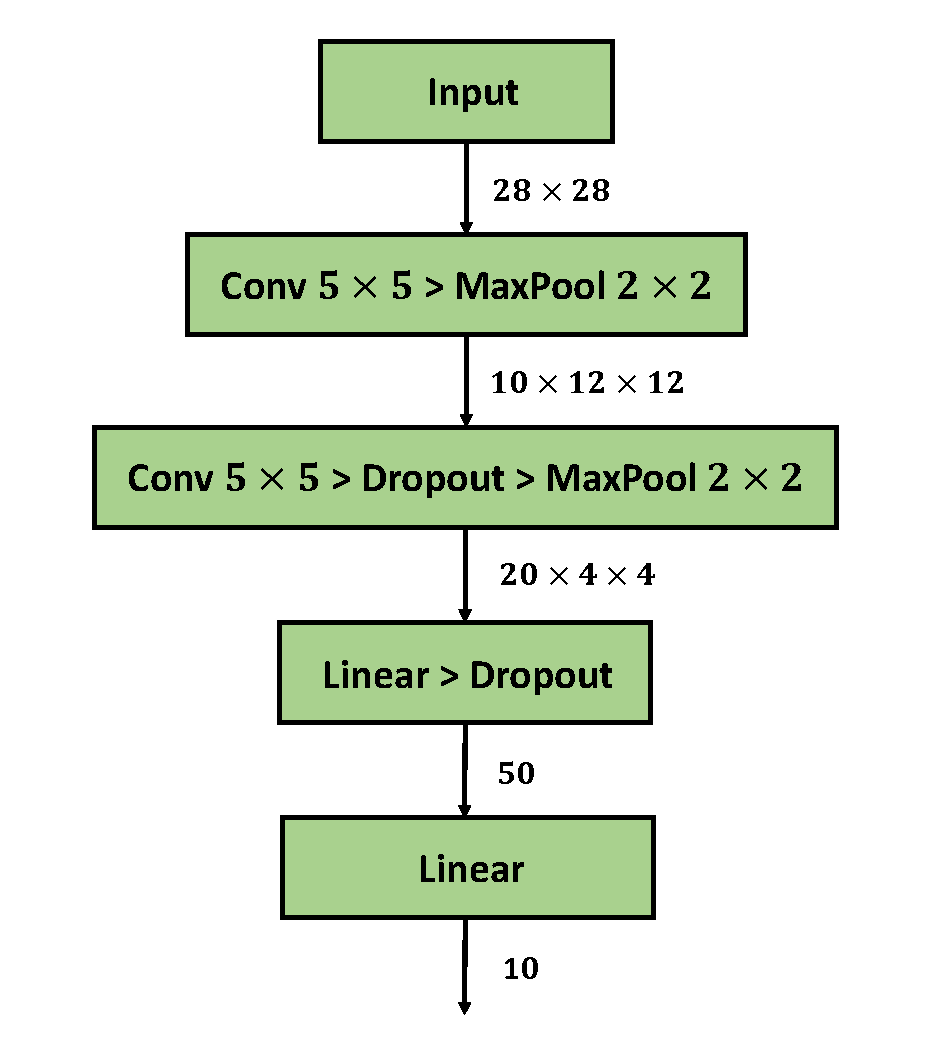
\includegraphics[width=1.95in]{plot/mnist_arch.pdf}\hspace{-0.1in}
        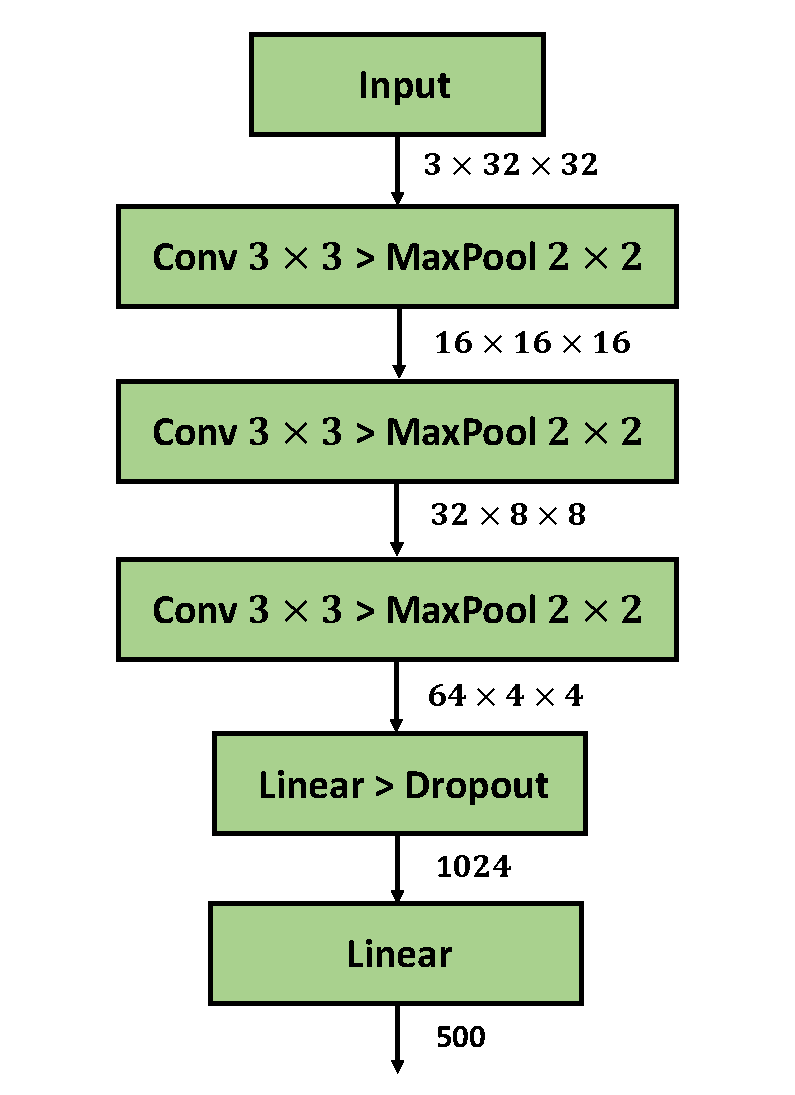
\includegraphics[width=1.95in]{plot/cifar_arch.pdf}
        \hspace{-0.1in}
        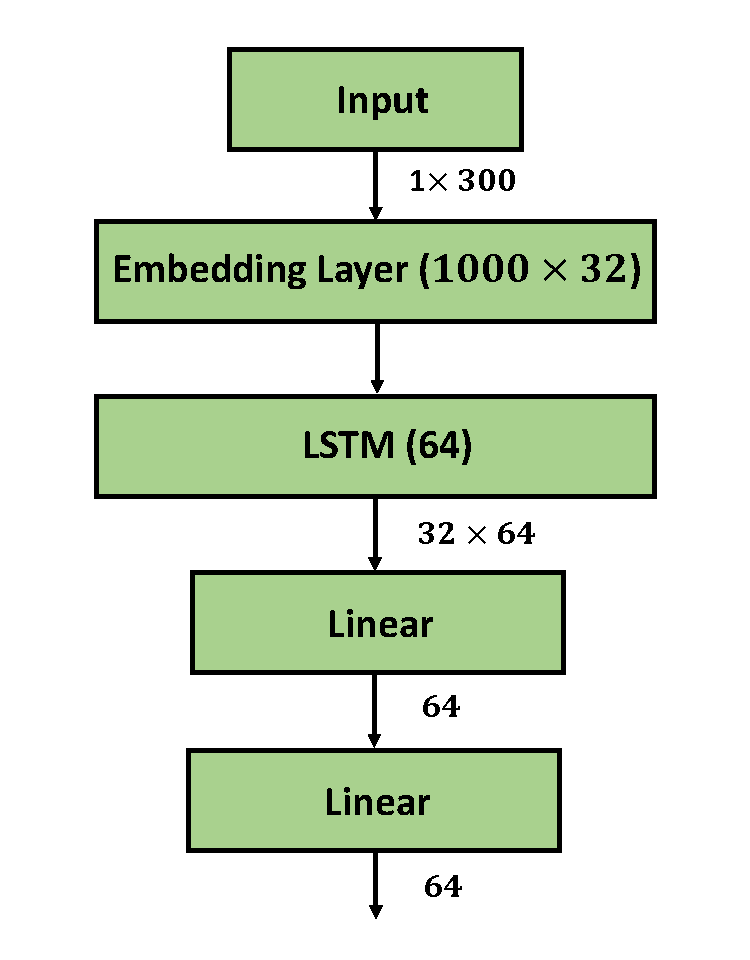
\includegraphics[width=1.95in]{plot/imdb_arch.pdf}
    }
    \end{center}
	\caption{Model architectures used in the experiments. Left: MNIST + CNN. Middle: CIFAR-10 + CNN. Right: IMDB + LSTM. In the last figure, the penultimate linear layer takes the last hidden state (64-dim vector) as the input.}
	\label{fig:model arch}
\end{figure}

In Figure~\ref{fig:model arch}, we provide the detailed description of the data and model architectures used in our numerical study. MNIST~\cite{mnist} is a popular hand-written letter recognition dataset, where each training sample is a $28\times 28$ black and white imagem each belonging to a class (digits 0-9). CIFAR-10~\cite{cifar} is a benchmark image classification dataset consisting of natural images from 10 classes. The image size is a $3\times 32\times 32$. In IMDB dataset, each sample is a movie review, and the task is to classify the reviews as positive or negative. The reviews are tokenized by words and transformed into integer vectors. We threshold at 300 for the length of each review. Zero-padding is applied to reviews that have less than 300 words. All our experiments are trained on GPU XXXXXXXXXX. We use two Convolutional Neural Networks (CNN) for MNIST and CIFAR-10. For IMDB dataset, we use a LSTM network. Each input movie review is a 300-dimensional vector, and the embedding layer embeds top 1000 most frequent words into 32-dimensional vectors. 64 LSTM cells are used, where the last hidden state is connected to two fully connected layers before the output.



\clearpage

\section{Additional content}\label{app:add}

\subsection{Extension to the single-machine setting}

We provide in this subsection the formulation of our method in the single-worker setting, see Algorithm~\ref{alg:sparsamssingle}.
Here, the computations, of the stochastic gradient and the various moment estimates, are all performed on a single-machine and the data is stored in this same worker.
Then, we establish its convergence rate with similar compression and error-feedback techniques, as seen prior.

\begin{algorithm}[H]
\caption{\algo\ with error-feedback for a single-machine} \label{alg:sparsamssingle}
\begin{algorithmic}[1]

\STATE \textbf{Input}: parameter $\beta_1$, $\beta_2$, learning rate $\eta_t$. 
\STATE Initialize: central server parameter $\theta_{1} \in \Theta \subseteq \mathbb R^d$; $e_{1}=0$ the error accumulator; sparsity parameter $k$; $m_0=0$, $v_0=0$, $\hat v_0=0$

\FOR{$t=1$ to $T$}
\STATE  Compute stochastic gradient $g_{t} \eqdef g_{t,i_t}$ at $\theta_t$ for randomly sampled index $i_t$ among the available observations indices. \label{line:stochgrad} 
\STATE  Compute $\tilde g_{t}=\textbf{Top-$k$}(g_{t}+e_{t},k)$ \label{line:topksingle} 
\STATE  Update the error $e_{t+1}=e_{t}+g_{t}-\tilde g_{t}$
\STATE $m_t=\beta_1 m_{t-1}+(1-\beta_1)\tilde g_t$
\STATE $v_t=\beta_2 v_{t-1}+(1-\beta_2)\tilde g_t^2$
\STATE $\hat v_t=\max(v_t,\hat v_{t-1})$ \label{line:vsingle}
\STATE Update the global model $\theta_{t+1}=\theta_{t}-\eta_t\frac{m_t}{\sqrt{\hat v_t+\epsilon}}$

\ENDFOR
\end{algorithmic}
\end{algorithm}


% ---------------------------------
% \begin{align*}
%     &\mathbb E[f(x_{t+1})]-f(x_t)\\
%     &\leq (-\frac{\eta}{C_0}+\frac{\eta^2 L}{\epsilon}+\frac{\eta \rho}{2\epsilon})\mathbb E[\|\nabla f(\theta_t)\|^2]+\frac{\eta^2 L \sigma^2}{n\epsilon}+\frac{\eta^3 C_1^2LG^2}{2\rho\epsilon}  \\
%     &\hspace{1in} + (\eta(1+C_1)G^2+\frac{\eta^2 (1+C_1)C_1LG^2}{\sqrt\epsilon})\mathbb E[\|D_t\|_1]+\eta^2C_1^2LG^2 \mathbb E[\|D_t\|^2].
% \end{align*}
% with $C_0\eqdef \sqrt{\frac{4(1+q^2)^3}{(1-q^2)^2}G^2+\epsilon}$. Setting $\eta\leq \frac{\epsilon}{4LC_0}$ and choosing $\rho=\frac{\epsilon}{2C_0}$, we obtain
% \begin{align*}
%     &\mathbb E[f(x_{t+1})]-f(x_t)\\
%     &\leq -\frac{\eta}{2C_0}\mathbb E[\|\nabla f(\theta_t)\|^2]+\frac{\eta^2 L \sigma^2}{n\epsilon}+\frac{\eta^3 C_0 C_1^2LG^2}{\epsilon^2}  \\
%     &\hspace{1in} + (\eta(1+C_1)G^2+\frac{\eta^2 (1+C_1)C_1LG^2}{\sqrt\epsilon})\mathbb E[\|D_t\|_1]+\eta^2C_1^2LG^2 \mathbb E[\|D_t\|^2].
% \end{align*}
% Summing over $t=1,...,T$, we get
% \begin{align*}
%     &\mathbb E[f(x_{T+1})-f(x_1)]\\
%     &\leq -\frac{\eta}{2C_0}\sum_{t=1}^T\mathbb E[\|\nabla f(\theta_t)\|^2]+\frac{T\eta^2 L \sigma^2}{n\epsilon}+\frac{T\eta^3 C_0 C_1^2LG^2}{\epsilon^2}  \\
%     &\hspace{1in} + (\eta(1+C_1)G^2+\frac{\eta^2 (1+C_1)C_1LG^2}{\sqrt\epsilon})\sum_{t=1}^T\mathbb E[\|D_t\|_1]+\eta^2C_1^2LG^2 \sum_{t=1}^T\mathbb E[\|D_t\|^2 \\
%     &\leq -\frac{\eta}{2C_0}\sum_{t=1}^T\mathbb E[\|\nabla f(\theta_t)\|^2]+\frac{T\eta^2 L \sigma^2}{n\epsilon}+\frac{T\eta^3 C_0 C_1^2LG^2}{\epsilon^2} + \frac{\eta (1+C_1)G^2d}{\sqrt\epsilon}+\frac{\eta^2 (1+2C_1)C_1LG^2d}{\epsilon},
% \end{align*}
% where the last inequality follows from Lemma~\ref{lemma:bound difference}. Re-arranging terms, we get that when $\eta\leq \frac{\epsilon}{4LC_0}$, 
% \begin{align*}
%     \frac{1}{T}\sum_{t=1}^T \mathbb E[\|\nabla f(\theta_t)\|^2]&\leq 2C_0\Big(\frac{\mathbb E[f(x_1')-f(x_{T+1}')]}{T\eta}+\frac{\eta L \sigma^2}{n\epsilon}+\frac{\eta^2 C_0 C_1^2LG^2}{\epsilon^2}\\
%     &\hspace{1.5in} + \frac{\eta (1+C_1)G^2d}{T\sqrt\epsilon}+\frac{\eta^2 (1+2C_1)C_1LG^2d}{T\epsilon} \Big)\\
%     &\leq 2C_0\Big(\frac{\mathbb E[f(\theta_1)-f(\theta^*)]}{T\eta}+\frac{\eta L \sigma^2}{n\epsilon}+\frac{\eta^2 C_0 C_1^2LG^2}{\epsilon^2}\\
%     &\hspace{1.5in} + \frac{\eta (1+C_1)G^2d}{T\sqrt\epsilon}+\frac{\eta^2 (1+2C_1)C_1LG^2d}{T\epsilon} \Big),
% \end{align*}
% where $C_0=\sqrt{\frac{4(1+q^2)^3}{(1-q^2)^2}G^2+\epsilon}$, $C_1=\frac{\beta_1}{1-\beta_1}+\frac{2q}{1-q^2}$, and the last inequality is because $\theta_1'=\theta_1$, and $\theta^* \eqdef \argmin_\theta f(\theta)$. This completes the proof.





%\section{Distributed setting Belhal}
%
%
%
%\subsection{Intermediary Lemmas}
%
%\begin{Lemma}\label{lem:bound}
%Under Assumption~\ref{ass:boundgrad} and Assumption~\ref{ass:var} we have for any iteration $t >0$:
%
%\begin{equation}
%\EE[\norm{m_t}^2] \leq (q^2+1) \sigma^2 \quad \textrm{and} \quad \EE[\hat v_t] \leq (q^2+1) \sigma^2
%\end{equation}
%where $m_t$ and $\hat v_t=\max(v_t,\hat v_{t-1})$ are defined Line~\ref{line:v} of Algorithm~\ref{alg:sparsams} and $\sigma^2 = \frac{1}{n}\sum_{i=1}^n  \sigma_i^2$.
%\end{Lemma}
%
%\begin{proof}
%We start by writing
%\begin{equation}
%\norm{\bar g_t}^2  = \norm{\frac{1}{n}\sum_{i=1}^n \tilde g_{t,i} }^2 \leq \frac{1}{n}\sum_{i=1}^n \norm{\tilde g_{t,i} }^2
%\end{equation}
%
%Though, using Assumption~\ref{ass:boundgrad} and Assumption~\ref{ass:var} we have:
%\begin{equation}
%\EE[\norm{\tilde g_{t,i} }^2]  = \EE[\norm{g_{t,i}  + \tilde g_{t,i}  - g_{t,i}}^2] \leq \EE[\norm{g_{t,i} }^2] + \EE[\norm{\tilde g_{t,i}  - g_{t,i}}^2] \leq (q^2+1)\sigma_i^2
%\end{equation}
%Hence
%\begin{equation}
%\EE[\norm{\bar g_t}^2]  \leq (q^2+1) \sigma^2
%\end{equation}
%where $\sigma^2 = \frac{1}{n}\sum_{i=1}^n  \sigma_{i}^2$.
%Then, by construction in Algorithm~\ref{alg:sparsams}:
%\begin{equation}
%\EE[\norm{m_t}^2]  \leq \beta_1^2 \EE[\norm{m_{t-1}}^2] + (1 - \beta_1)^2 \EE[\norm{\bar g_t}^2]  \leq \beta_1^2\EE[ \norm{m_{t-1}}^2] + (1 - \beta_1)^2(q^2+1) \sigma^2
%\end{equation}
%Since we have by initialization that $\norm{m_0}^2 \leq \sigma^2$, then we prove by induction that $\EE[\norm{m_t}^2] \leq (q^2+1) \sigma^2$.
%
%Similarly
%\begin{equation}
%\EE[\hat v_t] = \EE[\max(v_t,\hat v_{t-1})] = \max(\hat v_{t-1}, \beta_2 v_{t-1}+(1-\beta_2)\EE[\bar g_t^2]) \leq  \max(\hat v_{t-1}, \beta_2 v_{t-1}+(1-\beta_2)(q^2+1) \sigma^2) 
%\end{equation}
%\end{proof}
%
%\begin{Lemma}\label{lem:lemma1}
%Under Assumption~\ref{ass:smooth} to Assumption~\ref{ass:var}, with a decreasing sequence of stepsize $\{\eta_t\}_{t>0}$, we have:
%
%\begin{equation}
%-\eta_{t+1}\EE[\pscal{\nabla f(\theta_t)}{(\hat{V}_{t+1} + \epsilon \mathsf{I_d})^{-1/2} \bar{g}_t}] \leq - \frac{\eta_{t+1}}{2}  (\epsilon + \frac{(q^2+1)\sigma^2}{1 - \beta_2})^{-\frac{1}{2}} \EE[\norm{\nabla f(\theta_t)}^2] +q^2 \frac{\sigma^2 \eta_{t+1}}{\epsilon 2n^2}
%\end{equation}
%where $ \mathsf{I_d}$ is the identity matrix, $\hat{V_t}$ the diagonal matrix which diagonal entries are $\hat v_t=\max(v_t,\hat v_{t-1})$ defined Line~\ref{line:v} of Algorithm~\ref{alg:sparsams} and $\bar{g}_t$ is the aggregation of all \textbf{quantized} gradients from the workers.
%\end{Lemma}
%
%
%
%\begin{proof}
%We first decompose $\bar{g}_t$  as the sum of the unbiased stochastic gradients and its quantized versions as computed Line~\ref{line:topk} of Algorithm~\ref{alg:sparsams}:
%\begin{equation}
%\bar{g}_t = \frac{1}{n}\sum_{i=1}^n \tilde g_{t,i} = \frac{1}{n}\sum_{i=1}^n [ g_{t,i} + \tilde g_{t,i} - g_{t,i}]
%\end{equation}
%Hence,
%\begin{equation}
%\begin{split}
%T_1 := & -\eta_{t+1}\EE[\pscal{\nabla f(\theta_t)}{(\hat{V}_{t+1} + \epsilon \mathsf{I_d})^{-1/2} \bar{g}_t}] \\
%=  &\underbrace{ -\eta_{t+1}\EE[\pscal{\nabla f(\theta_t)}{(\hat{V}_{t+1} + \epsilon \mathsf{I_d})^{-1/2} \frac{1}{n}\sum_{i=1}^n  g_{t,i}} ]}_{t1} \underbrace{-\eta_{t+1}\EE[\pscal{\nabla f(\theta_t)}{(\hat{V}_{t+1} + \epsilon \mathsf{I_d})^{-1/2} \frac{1}{n}\sum_{i=1}^n  \tilde g_{t,i} - g_{t,i}}]}_{t_2}
%\end{split}
%\end{equation}
%
%\textbf{Bounding $t_1$:}
%Using the Tower rule, we have:
%\begin{equation}
%\begin{split}
%t_1 := &  -\eta_{t+1}\EE[\pscal{\nabla f(\theta_t)}{(\hat{V}_{t+1} + \epsilon \mathsf{I_d})^{-1/2} \frac{1}{n}\sum_{i=1}^n  g_{t,i}} ] \\
%=  & -\eta_{t+1}\EE[\EE[\pscal{\nabla f(\theta_t)}{(\hat{V}_{t+1} + \epsilon \mathsf{I_d})^{-1/2} \frac{1}{n}\sum_{i=1}^n  g_{t,i}} | \mathcal{F}_t]] \\
%=  & -\eta_{t+1}\EE[\pscal{\nabla f(\theta_t)}{(\hat{V}_{t+1} + \epsilon \mathsf{I_d})^{-1/2}\EE[ \frac{1}{n}\sum_{i=1}^n  g_{t,i}| \mathcal{F}_t]} ] 
%\end{split}
%\end{equation}
%Using Assumption~\ref{ass:boundgrad} and Lemma~\ref{lem:bound}, we have that 
%\begin{equation}\label{eq:lem2eq1}
%\begin{split}
%t_1 := &  -\eta_{t+1}\EE[\pscal{\nabla f(\theta_t)}{(\hat{V}_{t+1} + \epsilon \mathsf{I_d})^{-1/2} \frac{1}{n}\sum_{i=1}^n  g_{t,i}} ] \\
%\leq & - \eta_{t+1} (\epsilon + \frac{(q^2+1)\sigma^2}{1 - \beta_2})^{-\frac{1}{2}} \EE[\norm{\nabla f(\theta_t)}^2] 
% \end{split}
%\end{equation}
%
%
%\textbf{Bounding $t_2$:}
%
%We first recall Young's inequality with a constant $\delta \in (0,1)$ as follows:
%\begin{equation}\label{eq:young}
%\pscal{X}{Y} \leq \frac{1}{\delta} \|X\|^2 + \delta \|Y\|^2 \eqsp.
%\end{equation}
%
%Using Young's inequality \eqref{eq:young} with parameter equal to $1$:
%
%\begin{equation}\label{eq:lem2eq2}
%\begin{split}
%t_2 \leq &  \frac{\eta_{t+1}}{2} (\epsilon + \frac{(q^2+1)\sigma^2}{1 - \beta_2})^{-\frac{1}{2}} \EE[\norm{\nabla f(\theta_t)}^2] +\frac{\eta_{t+1}}{2n^2} \EE[\|(\hat{V}_{t+1} + \epsilon \mathsf{I_d})^{-1/2} \sum_{i=1}^n  \{ \tilde g_{t,i} - g_{t,i} \} \|^2]\\
%& \overset{(a)}{\leq} \frac{\eta_{t+1}}{2} (\epsilon + \frac{(q^2+1)\sigma^2}{1 - \beta_2})^{-\frac{1}{2}} \EE[\norm{\nabla f(\theta_t)}^2] +\frac{\eta_{t+1}}{2n^2} \EE[\|(\hat{V}_{t+1} + \epsilon \mathsf{I_d})^{-1/2} \|^2 \sum_{i=1}^n  \{\tilde g_{t,i} - g_{t,i} \} \|^2]\\
%& \overset{(b)}{\leq} \frac{\eta_{t+1}}{2} (\epsilon + \frac{(q^2+1)\sigma^2}{1 - \beta_2})^{-\frac{1}{2}} \EE[\norm{\nabla f(\theta_t)}^2] +\frac{\eta_{t+1}}{2n^2} \EE[\|(\hat{V}_{t+1} + \epsilon \mathsf{I_d})^{-1/2} \|^2] \EE[\| \sum_{i=1}^n  \{\tilde g_{t,i} - g_{t,i} \} \|^2]\\
%& \overset{(c)}{\leq} \frac{\eta_{t+1}}{2} (\epsilon + \frac{(q^2+1)\sigma^2}{1 - \beta_2})^{-\frac{1}{2}} \EE[\norm{\nabla f(\theta_t)}^2] +\frac{\eta_{t+1}}{\epsilon 2n^2}  \EE[\| \sum_{i=1}^n \tilde g_{t,i} - g_{t,i} \|^2]\\
%& \overset{(d)}{\leq} \frac{\eta_{t+1}}{2}(\epsilon + \frac{(q^2+1)\sigma^2}{1 - \beta_2})^{-\frac{1}{2}} \EE[\norm{\nabla f(\theta_t)}^2] +q^2\frac{\sigma^2 \eta_{t+1}}{\epsilon 2n^2}
%\end{split}
%\end{equation}
%where (a) uses the Cauchy-Schwartz inequality, (b) is due to the non-negativeness of both $\hat{V}_{t+1}$ and $\| \sum_{i=1}^n  \{g_{t,i} + \tilde g_{t,i} - g_{t,i} \} \|^2$ and (c) uses the Triangle inequality.
%We use Assumption~\ref{ass:quant} and Assumption~\ref{ass:var} in (d).
%
%Finally, combining \eqref{eq:lem2eq1} and \eqref{eq:lem2eq2} yields
%
%\begin{equation}
%-\eta_{t+1}\EE[\pscal{\nabla f(\theta_t)}{(\hat{V}_{t+1} + \epsilon \mathsf{I_d})^{-1/2} \bar{g}_t}] \leq - \frac{\eta_{t+1}}{2}  (\epsilon + \frac{(q^2+1)\sigma^2}{1 - \beta_2})^{-\frac{1}{2}} \EE[\norm{\nabla f(\theta_t)}^2] +q^2 \frac{\sigma^2 \eta_{t+1}}{\epsilon 2n^2}
%\end{equation}
%
%
%\end{proof}
%
%
%
%\begin{Lemma}\label{lem:lemma2}
%Under Assumption~\ref{ass:smooth} to Assumption~\ref{ass:var}, with a decreasing sequence of stepsize $\{\eta_t\}_{t>0}$, we have:
%
%\begin{equation}
%\begin{split}
%\EE[f(\theta_{t+1}) - f(\theta_{t}) ] \leq &   - \frac{\eta_{t+1}(1-\beta_1)}{2}  (\epsilon + \frac{(q^2+1)\sigma^2}{1 - \beta_2})^{-\frac{1}{2}} \EE[\norm{\nabla f(\theta_t)}^2] +q^2 \frac{G^2 \eta_{t+1}}{\epsilon 2n^2} \\
%&- \eta_{t+1} \beta_1\EE[\pscal{\nabla f(\theta_{t-1})}{(\hat{V}_{t} + \epsilon \mathsf{I_d})^{-1/2} m_{t}}]\\
%& +  \left(\frac{L}{2} + \beta_1 L \right) \norm{\theta_t - \theta_{t-1}}^2\\
%&+   \eta_{t+1} G^2 \EE[\sum_{j=1}^d \left[(\hat{v}^j_{t+1} + \epsilon )^{-1/2} - (\hat{v}^j_{t} + \epsilon )^{-1/2}  \right] ]
%\end{split}
%\end{equation}
%where $d$ denotes the dimension of the parameter vector
%\end{Lemma}
%
%
%
%\begin{proof}
%
%
%
%
%
%%Denote the following auxiliary variables at iteration $t+1$
%%\begin{align}
%%z_{t+1} = \theta_{t+1} + \frac{\beta_1}{1-\beta_1}(\theta_{t+1} - \theta_{t})
%%\end{align}
%
%By assumption Assumption~\ref{ass:smooth}, we can write the smoothness condition on the overall objective \eqref{eq:obj}, between iteration $t$ and $t+1$:
%
%\begin{equation}
%f(\theta_{t+1}) \leq f(\theta_{t})+  \pscal{\nabla f(\theta_t)}{\theta_{t+1} - \theta_{t}} + \frac{L}{2} \norm{\theta_{t+1} - \theta_{t}}^2
%\end{equation}
%
%Denote by $\hat{V_t}$ the diagonal matrix which diagonal entries are $\hat v_t=\max(v_t,\hat v_{t-1})$ defined Line~\ref{line:v} of Algorithm~\ref{alg:sparsams}.
%Hence, we obtain,
%\begin{equation}
%f(\theta_{t+1}) \leq f(\theta_{t}) - \eta_{t+1} \pscal{\nabla f(\theta_t)}{(\hat{V}_{t+1} + \epsilon \mathsf{I_d})^{-1/2} m_{t+1}} + \frac{L}{2} \norm{\theta_{t+1} - \theta_{t}}^2
%\end{equation}
%where $\mathsf{I_d}$ denotes the identity matrix.
%
%We now take the expectation of those various terms conditioned on the filtration $\mathcal{F}_t$ of the total randomness up to iteration $t$.
%\begin{equation}\label{eq:smooth1}
%\EE[f(\theta_{t+1}) - f(\theta_{t}) ] \leq - \eta_{t+1} \EE[\pscal{\nabla f(\theta_t)}{(\hat{V}_{t+1} + \epsilon \mathsf{I_d})^{-1/2} m_{t+1}}] + \frac{L}{2} \EE[\norm{\theta_{t+1} - \theta_{t}}^2]
%\end{equation}
%
%We now focus on the computation of the inner product obtained in the equation above.
%We have
%\begin{align}
%& \eta_{t+1}\EE[ \pscal{\nabla f(\theta_t)}{(\hat{V}_{t+1} + \epsilon \mathsf{I_d})^{-1/2} m_{t+1}}]  \label{innerprod}\\
%  = &\eta_{t+1} \EE[\pscal{\nabla f(\theta_t)}{(\hat{V}_{t+1} + \epsilon \mathsf{I_d})^{-1/2} m_{t+1} + (\hat{V}_{t} + \epsilon \mathsf{I_d})^{-1/2} m_{t+1} - (\hat{V}_{t} + \epsilon \mathsf{I_d})^{-1/2} m_{t+1}} ]\notag\\
%    = & \eta_{t+1}\EE[ \pscal{\nabla f(\theta_t)}{(\hat{V}_{t} + \epsilon \mathsf{I_d})^{-1/2} m_{t+1}} ] +  \eta_{t+1} \EE[\pscal{\nabla f(\theta_t)}{\left[(\hat{V}_{t+1} + \epsilon \mathsf{I_d})^{-1/2} - (\hat{V}_{t} + \epsilon \mathsf{I_d})^{-1/2}  \right]m_{t+1}}]\notag\\
% = & \eta_{t+1}\beta_1\EE[ \pscal{\nabla f(\theta_t)}{(\hat{V}_{t} + \epsilon \mathsf{I_d})^{-1/2} m_{t}}] +  \eta_{t+1} (1-\beta_1) \EE[\pscal{\nabla f(\theta_t)}{(\hat{V}_{t+1} + \epsilon \mathsf{I_d})^{-1/2} \bar{g}_t}] \notag\\
%&+  \eta_{t+1} \EE[\pscal{\nabla f(\theta_t)}{\left[(\hat{V}_{t+1} + \epsilon \mathsf{I_d})^{-1/2} - (\hat{V}_{t} + \epsilon \mathsf{I_d})^{-1/2}  \right]m_{t+1}}] \label{decomp}
%\end{align}
%where $\bar{g}_t$ is the aggregated gradients from all workers.
%
%Plugging the above in \eqref{eq:smooth1} yields:
%\begin{equation}\label{eq:main1}
%\begin{split}
%&\EE[f(\theta_{t+1}) - f(\theta_{t}) ] \\
%\leq & \underbrace{- \beta_1\EE[ \pscal{\nabla f(\theta_t)}{(\hat{V}_{t} + \epsilon \mathsf{I_d})^{-1/2} m_{t}}]}_{A_t} \eta_{t+1}\\
%& \underbrace{-  \EE[\pscal{\nabla f(\theta_t)}{\left[(\hat{V}_{t+1} + \epsilon \mathsf{I_d})^{-1/2} - (\hat{V}_{t} + \epsilon \mathsf{I_d})^{-1/2}  \right]m_{t+1}}]}_{B_t}\eta_{t+1}\\
%& \underbrace{-  (1-\beta_1) \EE[\pscal{\nabla f(\theta_t)}{(\hat{V}_{t+1} + \epsilon \mathsf{I_d})^{-1/2} \bar{g}_t}]}_{C_t} \eta_{t+1}+ \frac{L}{2} \EE[\norm{\theta_{t+1} - \theta_{t}}^2]
%\end{split}
%\end{equation}
%To begin with, by the tower rule, we have that 
%\begin{align}
%A_t & = - \beta_1\EE[\EE[\pscal{\nabla f(\theta_t)}{(\hat{V}_{t} + \epsilon \mathsf{I_d})^{-1/2} m_{t}}| \mathcal{F}_t]] \\
%& = - \beta_1 \pscal{\nabla f(\theta_{t-1})}{(\hat{V}_{t} + \epsilon \mathsf{I_d})^{-1/2} m_{t}}] - \beta_1 \pscal{\nabla f(\theta_t) - \nabla f(\theta_{t-1})}{(\hat{V}_{t} + \epsilon \mathsf{I_d})^{-1/2} m_{t}}]\\
%\end{align}
%where we recognize the first term as the term in \eqref{innerprod}, at iteration $t-1$ and hence apply the same decomposition as in \eqref{decomp}.
%Coupling with the smoothness of $f$, which gives that
%$$
%- \beta_1 \pscal{\nabla f(\theta_t) - \nabla f(\theta_{t-1})}{(\hat{V}_{t} + \epsilon \mathsf{I_d})^{-1/2} m_{t}}] \leq \frac{\beta_1 L}{\eta_{t-1}} \norm{\theta_t - \theta_{t-1}}^2
%$$
%
%we obtain,
%\begin{equation}\label{eq:termA}
%\begin{split}
%A_t & = - \beta_1\EE[\EE[\pscal{\nabla f(\theta_t)}{(\hat{V}_{t} + \epsilon \mathsf{I_d})^{-1/2} m_{t}}| \mathcal{F}_t]]\\
%&  \leq \eta_{t+1} \beta_1(A_{t-1} + B_{t-1} + C_{t-1})  + \eta_{t+1}\frac{\beta_1 L}{\eta_{t-1}} \norm{\theta_t - \theta_{t-1}}^2
%\end{split}
%\end{equation}
%Then,
%\begin{equation}\label{eq:termB}
%\begin{split}
%B_t & =-  \EE[\pscal{\nabla f(\theta_t)}{\left[(\hat{V}_{t+1} + \epsilon \mathsf{I_d})^{-1/2} - (\hat{V}_{t} + \epsilon \mathsf{I_d})^{-1/2}  \right]m_{t+1}}]\\
%& =  \EE[\sum_{j=1}^d  \nabla^j f(\theta_t)m_{t+1}^j \left[(\hat{v}^j_{t} + \epsilon )^{-1/2} - (\hat{v}^j_{t+1} + \epsilon )^{-1/2}  \right] ]\\
%& \overset{(a)}{\leq}  \EE[\norm{\nabla f(\theta_t)} \norm{m_{t+1}}\sum_{j=1}^d\left[(\hat{v}^j_{t} + \epsilon )^{-1/2} - (\hat{v}^j_{t+1} + \epsilon )^{-1/2}  \right] ]\\
%& \overset{(b)}{\leq}  G^2 \EE[\sum_{j=1}^d \left[(\hat{v}^j_{t} + \epsilon )^{-1/2} - (\hat{v}^j_{t+1} + \epsilon )^{-1/2}  \right] ]
%\end{split}
%\end{equation}
%where $\nabla^j f(\theta_t)$ denotes the j-th component of the gradient vector $\nabla f(\theta_t)$, (a) uses of the Cauchy-Schwartz inequality and (b) boils down from the norm of the gradient vector boundedness assumption \ref{ass:boundgrad}, denoting $G^2 \eqdef \frac{1}{n}\sum_{i=1}^n G_i^2$.
%
%
%Plugging the above into \eqref{eq:main1} yields
%\begin{equation}
%\begin{split}
%\EE[f(\theta_{t+1}) - f(\theta_{t}) ] \leq & \eta_{t+1}(A_t + B_t + C_t) + \frac{L}{2} \EE[\norm{\theta_{t+1} - \theta_{t}}^2]\\
% \leq &- \eta_{t+1} \beta_1\EE[\pscal{\nabla f(\theta_{t-1})}{(\hat{V}_{t} + \epsilon \mathsf{I_d})^{-1/2} m_{t}}]\\
%&+   \eta_{t+1} G^2 \EE[\sum_{j=1}^d \left[(\hat{v}^j_{t+1} + \epsilon )^{-1/2} - (\hat{v}^j_{t} + \epsilon )^{-1/2}  \right] ]\\
%&+  \left(\frac{L}{2} + \eta_{t+1}\frac{\beta_1 L}{\eta_{t-1}} \right) \norm{\theta_t - \theta_{t-1}}^2\\
%&-   \eta_{t+1}(1-\beta_1) \EE[\pscal{\nabla f(\theta_t)}{(\hat{V}_{t+1} + \epsilon \mathsf{I_d})^{-1/2} \bar{g}_t}]
%\end{split}
%\end{equation}
%
%We bound the last term on the RHS, $ -\eta_{t+1} \EE[\pscal{\nabla f(\theta_t)}{(\hat{V}_{t+1} + \epsilon \mathsf{I_d})^{-1/2} \bar{g}_t}]$ with Lemma~\ref{lem:lemma1}
%
%Under the assumption that we use a decreasing stepsize such that $\eta_{t+1} \leq \eta_{t}$, and given that according to Line~\ref{line:v} we have that $\hat v_{t+1} \geq \hat v_{t}$ by construction, we obtain 
%\begin{equation}
%\begin{split}
%\EE[f(\theta_{t+1}) - f(\theta_{t}) ] \leq &   - \frac{\eta_{t+1}(1-\beta_1)}{2}  (\epsilon + \frac{\frac{4(1+q^2)^3}{(1-q^2)^2}G^2}{1 - \beta_2})^{-\frac{1}{2}} \EE[\norm{\nabla f(\theta_t)}^2] +q^2 \frac{G^2 \eta_{t+1}}{\epsilon 2n^2} \\
%&- \eta_{t+1} \beta_1\EE[\pscal{\nabla f(\theta_{t-1})}{(\hat{V}_{t} + \epsilon \mathsf{I_d})^{-1/2} m_{t}}]\\
%& +  \left(\frac{L}{2} + \beta_1 L \right) \norm{\theta_t - \theta_{t-1}}^2\\
%&+   \eta_{t+1} G^2 \EE[\sum_{j=1}^d \left[(\hat{v}^j_{t+1} + \epsilon )^{-1/2} - (\hat{v}^j_{t} + \epsilon )^{-1/2}  \right] ]
%\end{split}
%\end{equation}
%
%Finally, using Lemma~\ref{lem:lemma1}, we obtain the desired result.
%\end{proof}
%
%
%
%\subsection{Proof of Theorem~\ref{thm:mainmultiple}}
%
%
%\begin{Theorem*}
%Under Assumption~\ref{ass:smooth} to Assumption~\ref{ass:var}, with a constant stepsize $\eta_t = \eta = \frac{L}{\sqrt{\maxiter}}$, we have:
%
%\begin{equation}
%\begin{split}
% \frac{1}{\maxiter}\sum_{t=1}^{\maxiter} \EE[\norm{\nabla f(\theta_t)}^2] \leq \frac{\EE[ f(\theta_{1}) - f(\theta_{\maxiter+1})]}{L \Delta_1 \sqrt{\maxiter}} + 
%d\frac{L \Delta_3}{\Delta_1 \sqrt{\maxiter}}  + \frac{\Delta_2}{\eta \Delta_1\maxiter} +\frac{1-\beta_1}{\Delta_1}  \epsilon^{-\frac{1}{2}} \sqrt{(q^2+1)}\sigma^2 
%\end{split}
%\end{equation}
%
%where 
%\begin{equation}
%\begin{split}
%\Delta_1 & \eqdef \frac{(1-\beta_1)}{2} (\epsilon + \frac{(q^2+1)\sigma^2}{1 - \beta_2})^{-\frac{1}{2}} \quad \textrm{,} \quad \Delta_2 \eqdef q^2 + \sum_{k=t+1}^\infty  \beta_1^{k-t+2}\frac{G^2 }{\epsilon 2n^2}\\
%\Delta_3 &\eqdef \left(\frac{L}{2} + 1+ \frac{\beta_1L}{1-\beta_1} \right) (1-\beta_2)^{-1} (1 - \frac{\beta_1^{2}}{\beta_2})^{-1}
%\end{split}
%\end{equation}
%\end{Theorem*}
%
%
%
%\begin{proof}
%
%
%By Lemma~\ref{lem:lemma2} we have 
%\begin{equation}
%\begin{split}
%\EE[f(\theta_{t+1}) - f(\theta_{t}) ] \leq &   - \frac{\eta_{t+1}(1-\beta_1)}{2}  (\epsilon + \frac{\frac{4(1+q^2)^3}{(1-q^2)^2}G^2}{1 - \beta_2})^{-\frac{1}{2}} \EE[\norm{\nabla f(\theta_t)}^2] +q^2 \frac{G^2 \eta_{t+1}}{\epsilon 2n^2} \\
%&- \eta_{t+1} \beta_1\EE[\pscal{\nabla f(\theta_{t-1})}{(\hat{V}_{t} + \epsilon \mathsf{I_d})^{-1/2} m_{t}}]\\
%& +  \left(\frac{L}{2} + \beta_1 L \right) \norm{\theta_t - \theta_{t-1}}^2\\
%&+   \eta_{t+1} G^2 \EE[\sum_{j=1}^d \left[(\hat{v}^j_{t+1} + \epsilon )^{-1/2} - (\hat{v}^j_{t} + \epsilon )^{-1/2}  \right] ]
%\end{split}
%\end{equation}
%
%Let us consider the following sequence, defined for all $t >0$:
%\beq\label{eq:defR}
%R_t \eqdef f(\theta_{t}) - \sum_{k=t}^\infty \eta_{k} \beta_1^{k-t+1}\EE[\pscal{\nabla f(\theta_{t-1})}{(\hat{V}_{t} + \epsilon \mathsf{I_d})^{-1/2} m_{t}}]
%\eeq
%
%We compute the following expectation:
%\begin{equation}
%\begin{split}
%\EE[R_{t+1}] - \EE[R_t] =& \EE[f(\theta_{t+1}) - f(\theta_{t}) ]  -  \sum_{k=t+1}^\infty \eta_{k} \beta_1^{k-t+2}\EE[\pscal{\nabla f(\theta_{t})}{(\hat{V}_{t+1} + \epsilon \mathsf{I_d})^{-1/2} m_{t+1}}] \\
%& +  \sum_{k=t}^\infty \eta_{k} \beta_1^{k-t+1}\EE[\pscal{\nabla f(\theta_{t-1})}{(\hat{V}_{t} + \epsilon \mathsf{I_d})^{-1/2} m_{t}}]\\
%\end{split}
%\end{equation}
%
%Using the Assumption~\ref{ass:smooth}, we note that:
%\begin{equation}
%\begin{split}
%\EE[f(\theta_{t+1}) - f(\theta_{t}) ] \leq - \eta_{t+1} \EE[\pscal{\nabla f(\theta_{t})}{(\hat{V}_{t+1} + \epsilon \mathsf{I_d})^{-1/2} m_{t+1}}] +\frac{L}{2}  \norm{\theta_{t+1} - \theta_{t}}^2
%\end{split}
%\end{equation}
%which yields
%\begin{equation}
%\begin{split}
%\EE[R_{t+1}] - \EE[R_t] =& - (\eta_{t+1} + \sum_{k=t+1}^\infty \eta_{k} \beta_1^{k-t+2})\EE[\pscal{\nabla f(\theta_{t})}{(\hat{V}_{t+1} + \epsilon \mathsf{I_d})^{-1/2} m_{t+1}}] \\
%& +  \sum_{k=t}^\infty \eta_{k} \beta_1^{k-t+1}\EE[\pscal{\nabla f(\theta_{t-1})}{(\hat{V}_{t} + \epsilon \mathsf{I_d})^{-1/2} m_{t}}]\\
%& +\frac{L}{2}  \norm{\theta_{t+1} - \theta_{t}}^2\\
%\leq&  (\eta_{t+1} + \sum_{k=t+1}^\infty \eta_{k} \beta_1^{k-t+2})\EE[A_t + B_t + C_t] \\
%& -  \sum_{k=t}^\infty \eta_{k} \beta_1^{k-t+1}\EE[A_{t-1} + B_{t-1} + C_{t-1}]\\
%& +\frac{L}{2}  \norm{\theta_{t+1} - \theta_{t}}^2
%\end{split}
%\end{equation}
%
%where $A_t, B_t, C_t$ are defined in \eqref{eq:main1}.
%
%We use \eqref{eq:termA} and \eqref{eq:termB} to bound $A_t$ and $B_t$, and Lemma~\ref{lem:lemma1} to bound $C_t$ where we precise that the learning rate $\eta_{t+1}$ becomes $ \eta_{t+1}+ \sum_{k=t+1}^\infty \eta_{k} \beta_1^{k-t+2}$.
%Hence
%\begin{equation}\label{eq:mainR}
%\begin{split}
%\EE[R_{t+1}] - \EE[R_t] \leq &
%  \left( (\eta_{t+1} + \sum_{k=t+1}^\infty \eta_{k} \beta_1^{k-t+2}) \beta_1- \sum_{k=t}^\infty \eta_{k} \beta_1^{k-t+1}\right) \EE[A_{t-1} + B_{t-1} + C_{t-1}]\\
%&  +  (\eta_{t+1}+ \sum_{k=t+1}^\infty \eta_{k} \beta_1^{k-t+2}) G^2 \EE[\sum_{j=1}^d \left[(\hat{v}^j_{t+1} + \epsilon )^{-1/2} - (\hat{v}^j_{t} + \epsilon )^{-1/2}  \right] ]\\
%& + \left(\frac{L}{2} + (\eta_{t+1}+ \sum_{k=t+1}^\infty \eta_{k} \beta_1^{k-t+2})\frac{\beta_1 L}{\eta_{t-1}} \right)   \norm{\theta_{t+1} - \theta_{t}}^2\\
%& - (\eta_{t+1}+ \sum_{k=t+1}^\infty \eta_{k} \beta_1^{k-t+2})\frac{(1-\beta_1)}{2}  (\epsilon + \frac{(q^2+1)\sigma^2}{1 - \beta_2})^{-\frac{1}{2}} \EE[\norm{\nabla f(\theta_t)}^2] \\
%& +q^2 \eta_{t+1}+ \sum_{k=t+1}^\infty \eta_{k} \beta_1^{k-t+2}\frac{G^2 }{\epsilon 2n^2}
%\end{split}
%\end{equation}
%where the last term in the LHS is due to Lemma~\ref{lem:lemma2}.
%
%By assumption, we have that for all $t >0$, $\eta_{t=1} \leq \eta_t$.
%Also, set the tuning parameters such that
%\begin{equation}
% \eta_{t}+ \sum_{k=t}^\infty \eta_{k} \beta_1^{k-t+1} \leq \frac{\eta_t}{1 - \beta_1}
% \end{equation}
% so that 
%\begin{equation}
%\begin{split}
%& (\eta_{t+1} + \sum_{k=t+1}^\infty \eta_{k} \beta_1^{k-t+2}) \beta_1- \sum_{k=t}^\infty \eta_{k} \beta_1^{k-t+1} = 0\\
%\iff& (\eta_{t+1} + \sum_{k=t+1}^\infty \eta_{k} \beta_1^{k-t+2}) \beta_1 = \sum_{k=t}^\infty \eta_{k} \beta_1^{k-t+1}
%\end{split}
%\end{equation}
%
%Note that $- (\eta_{t+1}+ \sum_{k=t+1}^\infty \eta_{k} \beta_1^{k-t+2})\frac{(1-\beta_1)}{2}  (\epsilon + \frac{\frac{4(1+q^2)^3}{(1-q^2)^2}G^2}{1 - \beta_2})^{-\frac{1}{2}}\leq - \eta_{t+1}\frac{(1-\beta_1)}{2} (\epsilon + \frac{\frac{4(1+q^2)^3}{(1-q^2)^2}G^2}{1 - \beta_2})^{-\frac{1}{2}}$ since $ \sum_{k=t+1}^\infty \eta_{k} \beta_1^{k-t+2} \geq 0$.
%
%The above coupled with \eqref{eq:mainR} yields
%
%\begin{equation}\label{eq:mainR2}
%\begin{split}
%\EE[R_{t+1}] - \EE[R_t] \leq & - \eta_{t+1}\frac{(1-\beta_1)}{2} (\epsilon + \frac{\frac{4(1+q^2)^3}{(1-q^2)^2}G^2}{1 - \beta_2})^{-\frac{1}{2}} \EE[\norm{\nabla f(\theta_t)}^2]+q^2 \eta_{t+1}+ \sum_{k=t+1}^\infty \eta_{k} \beta_1^{k-t+2}\frac{G^2 }{\epsilon 2n^2}\\
%&  -  (\eta_{t+1}+ \sum_{k=t+1}^\infty \eta_{k} \beta_1^{k-t+2}) G^2 \EE[\sum_{j=1}^d \left[(\hat{v}^j_{t} + \epsilon )^{-1/2} - (\hat{v}^j_{t+1} + \epsilon )^{-1/2}  \right] ]\\
%& + \left(\frac{L}{2} + 1+ \frac{\beta_1L}{1-\beta_1} \right)  \EE[ \norm{\theta_{t+1} - \theta_{t}}^2]
%\end{split}
%\end{equation}
%
%We now sum from $t = 1$ to $t = \maxiter$  the inequality in \eqref{eq:mainR2}, and divide it by $\maxiter$:
%
%\begin{equation}\label{eq:finalR2}
%\begin{split}
%&\eta\frac{(1-\beta_1)}{2} (\epsilon + \frac{\frac{4(1+q^2)^3}{(1-q^2)^2}G^2}{1 - \beta_2})^{-\frac{1}{2}} \frac{1}{\maxiter}\sum_{t=1}^{\maxiter} \EE[\norm{\nabla f(\theta_t)}^2] \\
%\leq & \frac{\EE[R_1] - \EE[R_{\maxiter+1}]}{\maxiter} + \frac{q^2 \eta+ \sum_{k=t+1}^\infty \eta \beta_1^{k-t+2}\frac{G^2 }{\epsilon 2n^2}}{\maxiter}\\
%& + \left(\frac{L}{2} + 1+ \frac{\beta_1L}{1-\beta_1} \right)\frac{1}{\maxiter}  \sum_{t=1}^{\maxiter}\EE[ \norm{\theta_{t+1} - \theta_{t}}^2]
%\end{split}
%\end{equation}
%
%where we have used the fact that $(\hat{v}^j_{t} + \epsilon )^{-1/2} - (\hat{v}^j_{t+1} + \epsilon )^{-1/2} \geq 0$ for all dimension $j \in [d]$ by construction of $\hat{v}^j_{t+1}$.
%
%We now bound the two remaining terms:
%
%
%\textbf{Bounding $-\EE[R_{\maxiter+1}]$:}
%
%By definition \eqref{eq:defR} of $R_t$ we have, using Lemma~\ref{lem:bound}:
%\beq
%\begin{split}
%-\EE[R_{\maxiter+1}] \leq & \sum_{k=T+1}^\infty \eta_{k} \beta_1^{k-t+1}\EE[\pscal{\nabla f(\theta_{t-1})}{(\hat{V}_{t} + \epsilon \mathsf{I_d})^{-1/2} m_{t}}] - f(\theta_{\maxiter+1})\\
%& \leq\| \sum_{k=T+1}^\infty \eta_{k} \beta_1^{k-t+1}\| \|\nabla f(\theta_{t-1})\| \|(\hat{V}_{t} + \epsilon \mathsf{I_d})^{-1/2} m_{t}\|\\
%& \leq \eta_{t+1} (1-\beta_1) \epsilon^{-\frac{1}{2}} \sqrt{(q^2+1)}\sigma^2 - f(\theta_{\maxiter+1})
%\end{split}
%\eeq
%
%
%
%
%
%
%\textbf{Bounding $   \sum_{t=1}^{\maxiter }\EE[ \norm{\theta_{t+1} - \theta_{t}}^2]$:}
%
%By definition in Algorithm~\ref{alg:sparsams}:
%
%\begin{equation}\label{eq:gap}
%\begin{split}
%\norm{\theta_{t+1} - \theta_{t}}^2  = \eta_{t+1}^2 \left[ (\hat V_{t+1}+\epsilon \mathsf{I_d})^{-\frac{1}{2}} m_{t+1}\right]^2 = \eta_{t+1}^2 \sum_{j=1}^d  \frac{|m_{t+1}^j|^2}{\hat{v}^j_{t+1} + \epsilon}
%\end{split}
%\end{equation}
%
%For any dimension $j \in [d]$,
%\begin{equation}
%\begin{split}
%|m_{t+1}^j|^2 &= |\beta_1 m_{t}^j + (1-\beta_1) \bar g_t^j |^2\\
%& \leq \beta_1(\beta_1^2 |m_{t-1}^j|^2 + (1-\beta_1)^2 |\bar g_{t-1}^j|^2) +  |\bar g_t^j|^2\\
%& \leq \sum_{k=0}^t \beta_1^{2(t-k)}|\bar g_k^j|^2\\
%& \leq \sum_{k=0}^t \frac{\beta_1^{2(t-k)}}{\beta_2^{t-k}}\beta_2^{t-k}|\bar g_k^j|^2
%\end{split}
%\end{equation}
%
%Using Cauchy-Schwartz inequality we obtain
%\begin{equation}\label{eq:temp1}
%\begin{split}
%|m_{t+1}^j|^2  \leq \sum_{k=0}^t \frac{\beta_1^{2(t-k)}}{\beta_2^{t-k}}\beta_2^{t-k}|\bar g_k^j|^2 &\leq \sum_{k=0}^t \left(\frac{\beta_1^{2}}{\beta_2}\right)^{t-k}  \sum_{k=0}^t\beta_2^{t-k}|\bar g_k^j|^2\\
%&\leq \frac{1}{1 - \frac{\beta_1^{2}}{\beta_2}} \sum_{k=0}^t\beta_2^{t-k}|\bar g_k^j|^2
%\end{split}
%\end{equation}
%
%On the other hand we have
%\begin{equation}
%\hat{v}^j_{t+1} \geq \beta_2 \hat{v}^j_{t} + (1-\beta_2) (\bar g_t^j)^2
%\end{equation}
%and since it is also true for iteration $t=1$, we have by induction replacing $v_t^j$ in the above that 
%\begin{equation}\label{eq:temp2}
%\begin{split}
%\hat{v}^j_{t+1} \geq (1-\beta_2) \sum_{k=0}^t\beta_2^{t-k}|\bar g_k^j|^2 \iff  \frac{\sum_{k=0}^t\beta_2^{t-k}|\bar g_k^j|^2}{ \hat{v}^j_{t+1}} \leq    (1-\beta_2)^{-1}
%\end{split}
%\end{equation}
%
%Hence, we can derive from \eqref{eq:gap} that
%
%\begin{equation}\label{eq:gap2}
%\begin{split}
%\norm{\theta_{t+1} - \theta_{t}}^2  = \eta_{t+1}^2 \sum_{j=1}^d  \frac{|m_{t+1}^j|^2}{\hat{v}^j_{t+1} + \epsilon}&\leq  \eta_{t+1}^2 \sum_{j=1}^d  \frac{|m_{t+1}^j|^2}{\hat{v}^j_{t+1}}\\
%&\overset{(a)}{\leq}   \eta_{t+1}^2 \sum_{j=1}^d  \frac{1}{1 - \frac{\beta_1^{2}}{\beta_2}} \frac{\sum_{k=0}^t\beta_2^{t-k}|\bar g_k^j|^2}{\hat{v}^j_{t+1}}\\
%&\overset{(b)}{\leq} \eta_{t+1}^2 d (1-\beta_2)^{-1} (1 - \frac{\beta_1^{2}}{\beta_2})^{-1}
%\end{split}
%\end{equation}
%where (a) uses \eqref{eq:temp1} and (b) uses \eqref{eq:temp2}.
%
%
%Plugging the two bounds in \eqref{eq:finalR2}, we obtain the following bound:
%
%\begin{equation}
%\begin{split}
% \frac{1}{\maxiter}\sum_{t=1}^{\maxiter } \EE[\norm{\nabla f(\theta_t)}^2] \leq & \frac{\EE[ f(\theta_{1}) - f(\theta_{\maxiter+1})]}{\eta \Delta_1 \maxiter} + \frac{q^2 \eta+ \sum_{k=t+1}^\infty \eta \beta_1^{k-t+2}\frac{G^2 }{\epsilon 2n^2}}{\eta \Delta_1\maxiter}\\
%&+\frac{1-\beta_1}{\Delta_1}  \epsilon^{-\frac{1}{2}} \sqrt{(q^2+1)}\sigma^2 \\
%& + \left(\frac{L}{2} + 1+ \frac{\beta_1L}{1-\beta_1} \right)\frac{1}{\eta \Delta_1}  \eta^2 d (1-\beta_2)^{-1} (1 - \frac{\beta_1^{2}}{\beta_2})^{-1}
%\end{split}
%\end{equation}
%
%
%where $\Delta_1 \eqdef \frac{(1-\beta_1)}{2} (\epsilon + \frac{(q^2+1)\sigma^2}{1 - \beta_2})^{-\frac{1}{2}}$
%
%With a constant stepsize $\eta = \frac{L}{\sqrt{\maxiter}}$ we get the final convergence bound as follows:
%\begin{equation}
%\begin{split}
% \frac{1}{\maxiter}\sum_{t=1}^{\maxiter} \EE[\norm{\nabla f(\theta_t)}^2] \leq & \frac{\EE[ f(\theta_{1}) - f(\theta_{\maxiter+1})]}{L \Delta_1 \sqrt{\maxiter}} + 
%d\frac{L \Delta_3}{\Delta_1 \sqrt{\maxiter}} \\
%& + \frac{\Delta_2}{ \Delta_1\maxiter} +\frac{1-\beta_1}{\Delta_1}  \epsilon^{-\frac{1}{2}} \sqrt{(q^2+1)}\sigma^2 
%\end{split}
%\end{equation}
%where $\Delta_2 \eqdef q^2 + \sum_{k=t+1}^\infty  \beta_1^{k-t+2}\frac{G^2 }{\epsilon 2n^2}$ and $\Delta_3 \eqdef \left(\frac{L}{2} + 1+ \frac{\beta_1L}{1-\beta_1} \right) (1-\beta_2)^{-1} (1 - \frac{\beta_1^{2}}{\beta_2})^{-1}$.
%
%
%\end{proof}
%
%
%
%\clearpage




\end{document} 
